\documentclass{article}
\usepackage[utf8]{inputenc}

\title{CCLtracker Framework: Monitoring users learning and activity in web based citizen science projects
}
\author{ Jose Luis Fernandez-Marquez, Ioannis Charalampidis,\\ Oula Abu-Amsha, Francois Grey, Brian Fuchs, \\ Daniel K. Schneider, Ben Segal, S.P. Mohanty, Egle Marija Ramanauskaite}
\date{July 2015}

\usepackage{natbib}
\usepackage{graphicx}
\usepackage{subfigure}

\begin{document}

\maketitle

\begin{abstract}
The explosion of web applications and on-line services over the last 20 years have made analytics tools highly required to understand who the users are, how they reach to the web site, and how they behave. That allows monitoring key performance indicators (e.g. downloads, sales, or participation on the web), improving users interfaces, planning, executing, and evaluating actions intended to increase users engagement. 

Measuring and improving users engagement in citizen science projects is not different from other web applications such as on-line shopping, newspapers, or sites for recommending music or movies. However, citizen science project usually lack the needed resources to implement a proper user monitoring system. Mainly, The lack of high-level API for implementing user monitoring in a reusable and modular way, induces huge development efforts.  

This paper presents CCLTracker analytics framework that is intended to overcome current analytics tool limitations, and providing an API for monitoring users activities such as time spent watching a video, time to complete a task, or how far a page is scrolled down (the percentage). The CCLTracker has been integrated in 3 different citizen science projects proving its value for measuring learning. 

\end{abstract}

\section{Introduction}

% \begin{itemize}
%     \item  Why web tracking exist? (motivation)
%     \item  Relation between web tracking for commercial applications and non-profit and citizen science projects. 
%     \item Why existing tools are not satisfying our requirements? (2 paragraphs summarizing the related work and explaining the lack of tools like CCL tracker. 
%     \item Impact. 
% \end{itemize}



The explosion of web applications and on-line services over the last 20 years have made analytics tools highly required to understand who the users are, how they find the web, and how they behave. That allows to monitor key performance indicators (e.g. downloads, sells, or participation on web), improve users interfaces, planing, execute, and evaluate actions to increase users engagement. 

A web based citizen science project is not  different than other online services. Dissemination actions are focused also on engaging users and empower their participation on the project. Citizen science projects require understand who are the users, where they are coming from, and how they behave in the website. Additionally, citizen science projects aim to provide learning outcomes. Unlike other web services, citizen science projects focus on two kind of indicators: (1) key performance indicator such as number of visitors, number of goals achieved (e.g. number of tasks developed by users), or number of clicks on links to external sources; and (2) key learning indicators such as accuracy of the task done, speed developing the task, \% of tutorial and extra contents accessed, or participation in forum or chats. Key performance and learning indicators can be measured using analytics data. 

There are a bunch of different analytics tools such as Google Analytics, and Piwik, which provide very interesting analytics information about the users, and the website. These tools store and aggregate the analytics data, and provide a Graphical User Interface (GUI) that allows users without programming skills to manipulate analytics data and create customs reports to periodically monitor key  indicators.  


However, the information regarding the user behaviour is limited to average time per session, pages views, or bound rate (i.e. percentage of people that leave the site without ant interaction). These information is not relevant for evaluating user participation in citizen science projects, neither to understands who are the people who really contribute. Even thought, analytics tools provide information about where the users are coming from, it is not enough to evaluate dissemination activities. E.g. we could observe than 500 users are coming from reddit, but if we do not know if they participate on the citizen science project. 


Monitoring key performance and learning indicators in a citizen science projects require to monitor the user behaviour.  Both tools, GA and Piwik allows to send application specific events, i.e. events designed to be fired from the website when monitoring users' specific actions. For example, we can add number of click per sessions, number of times an user writes on the forum, clicks to internal and external links, whether the user is scrolling down the web or how long time an user has been watching a video. All these examples require to program a tracking system in the client side and connect it with the analytics tool. This tracking system is tough to implement and keep it updated over the different version of the web. Additionally, it creates dependencies with the analytics tools.

This paper presents CCLTracker analytics framework to ease monitoring users behaviour in citizen science projects, overcoming current analytics tool limitations and reducing the implementation effort. The main contribution of this framework is a Java Script library that can be easily connected to other analytics tools, providing:

\begin{itemize}
\item Client side aggregation of data before sending it to the analytics tool (i.e. GA or Piwik). 
\item High level API to ease the creation and manipulation of events. 
\item Decoupling between the tracking system and the analytics tools. I.e. Event created from CCLTracker library can be sent to Google Analytics, Piwik or whatever analytics tool able to capture JS events. 
\end{itemize}


As a proof of concept this paper shows the CCLTracker analytics framework composed of Google Analytics, Google Tag Manager, and the CCLtracker JS library. We present detailed results from a case study and show how the framework overcomes current Google Analytics limitations. 
 
Section~\ref{sec:related} describes existing analtyics tools and their limitations. Section~\ref{CCLTracker} introduces the CCLTracker framework. A case study is presented in Section~\ref{sec:caseStudy}. Finally we present conclusions and future work. 
 

\section{Background}\label{sec:related}


% \begin{itemize}
% \item Existing frameworks and tools for web user tracking (Google Analytics, piwik, and existing papers. For each of them advantages and disadvantages. 
% \item Tracking client side. There are many papers. 
% \item Basically this section should conclude highlighting the novelty of CCLTracker on the state of the art. 
% \end{itemize}
   
   
There are two main web-based analytics tools, Google Analytics~\cite{} and Piwik~\cite{}. A major difference between then is that Piwik is open source and you can deploy it in a local environment, having full control, full access to the data, and privacy. On the other hand Google analytics is a free service provided by google, and the information is stored in their servers. Additionally, Google Analytics provides demographic information about the users such as, age, gender and interests. Both analytics tools provide information about the users in three categories: audience, acquisition, and behaviour.

\textbf{Audience} provides information about who the users are, and general information about the site performance such as number of users, number of sessions, page views, or average pages per session. Regarding the users we can gather information about their age, gender, location, their interest (affinity category and in-market segment), the browsers, mobile phones, operating systems, screen resolutions, or languages. 
   
\textbf{Acquisition} provides information about how the users reach the website. I.e. using the URL (direct), using a organic search, from a referral or social media. This information helps to evaluate dissemination activities.   

\textbf{Behaviour} provides information about what the user is doing in the website, e.g. pages visited, or behavior flow, and information about the site performance, e.g. Average page load time, or average server connection time. Additionally, this section provides information about user events. User events allow to track user activities within the website, but each of the events requires to be implemented in our website. Events are extremely important to understand what the user is doing in the website, everything can be tracked but it can involve a high complexity. E.g. Internal/external clicks, time spent between clicks, mouse trajectories, scroll down on the pages, time spent watching a video or listening an audio, etc. Events provide a very powerful tool for large scale debugging. Events can be user actions, but also system errors. Tracking system errors such as problem downloading a file, web service not available, or wrong email in the log in session, provide two main advantages. On one hand we can easily detect bugs that appear with very low frequency, i.e. 1/1000 or 1/10000. On the other hand, we can cross the information regarding the error with information coming from Google Analytics such as browser, Operative System, screen resolution, or Internet provider. Crossing those data, allows as to reproduce the errors and fix them using users as debuggers. Notice that this implementation requires an experienced programmer and it couples the website code with the analytic tool. It gets very tough to implement when we are using complex Java Script applications and it is difficult to maintain through out the application development cycles, i.e. little changes on the functional code of the application might make produce wrong analytics data.  

   
  
 
There are three major ways of manipulating data in GA: \textbf{Crossing, Segmenting and Filtering}. Google Analytics allows to cross data by adding a second dimension, e.g. we can see number of users per country, or number of session coming from Facebook per country. Segmentation allows us to focus the analytics data on a subset of sessions or users, e.g. users coming from Spain, new users, female users, users between 18 and 24 years old, users coming from Reddit. Filtering allows to clean the data and remove those that is not relevant. E.g. we could ask for all referrals order by bounce rate to know the user engagement from different referrals, however, we can find at the top referrals with few users that are not relevant for the stats. In this case we can apply a filter to remove from the list those referrals with less than a number of users. 



An interesting feature provide by GA is \textbf{Custom Reports}. Custom reports allow to create templates with aggregated data, applying crossing, segmentation and filtering. Custom reports are used to periodically monitor key performance indicators saving time on creating the aggregations. 


\subsection{Current limitations}

There two types of limitations in GA: limitations regarding data limits\footnote{https://support.google.com/analytics/answer/1070983?hl=en}, such as 10 million hits per month or 200,000 sessions per day. Those limitations maybe skipped by upgrading to Google Analytics Premium which has an associated cost, or using another analytic tools such as Piwik which is open source and there are not data limits. Notice that Piwik does not provide analytics data about the users' age, gender, or interest. Moreover, Piwik requires to be hosted and managed in our own servers. 

The second type of limitations refer to functional limitations. Most of existing limitations can be overcome by using external tools. For example, it is not possible to do cluster analysis or user profiling in GA. However, there are libraries for exporting data to R~\cite{} or services to export data in standard format such as Google Query Explorer\footnote{https://ga-dev-tools.appspot.com/query-explorer/}. Moreover, it is not possible to make analytics data public because the access to GA data requires authentication, in this case we can user Google Super Proxy\footnote{https://developers.google.com/analytics/solutions/google-analytics-super-proxy} which allow to create a proxy using your credential and provide the data using standard formats that can be visualised using APIs such as Google Charts\footnote{https://developers.google.com/chart/}.


One of the major limitations comes when we want to measure engagement or measuring some kind of user activity in our website. Information provided by GA regarding engagement is very poor, e.g. time per session, bounce rate, or pages views. For example an on-line shop would like to know about those people who buy, or those who leave the site without buying. In a citizen science project~\footnote{http://crowdcrafting.org/} it would be interesting who are the people contributing and who are those who visit the site but there are not participating, who are posting information on the forum, or who are playing a key role on the project. To get this data we need to use application specific events, i.e. events monitoring user activity on the web. In this case, developers need to implement it and release a new version of the site. Some times, specially in big companies, this new analytics requirements need to wait for the approval and the next official release. In order to mitigate this delay and make data scientist more independent from web developers, google released Google Tag Manager\footnote{http://www.google.com/tagmanager/} (GTM). GTM allows to add new tags (tracking new events) by using a graphical interface, and inject the code in the website without need to wait for developers to release the code. There many others tools and service that can be user to overcome limitations and extend GA functionality. That makes GA not a simply tool, but an eco-system of developers, tools, services, and users.

This paper describes how to mitigate the complexity of adding application specific events (i.e. tracking events) and decouple the dependency with Google Analytics or any other tracking tool, allowing to migrate to other tracking tools or having the tracking data replicated in a local server. Many companies are using google analytics and integrated tags in their tracking code, i.e. where user click, when they manage to sell a product, user profiling, or tracking user attention, however, that involves a huge developing effort, and once it is implemented the tracking code will be coupled to the analytics tool. For example, if we are using GA and we reach the data limit we will find to option: pay for a premium account or send fewer hits to GA. Migrating to another analytics tools such as Piwik or storing the data in a local server will involve a huge developing effort. Additionally, as far as we know there is not any library focusing on mitigating this effort, by providing a high level API to ease the implementation of application specific events. 


% I am not sure if we should mention the problem of advance segmentation. 


In this paper we propose CCLTracker library which provides a high level API for tracking events and decouple your tracking code from any analytics tool, thus allowing to easily migrate to another existing analytics tool or to store the application specific events locally. CCLtracker library is implemented in Java Script and integrated in the CCLTracker Framework (See section~\ref{sec:CCLtrackerFramerwork}). The CCL tracking framework is composerd by GA, Google Tag Manager (GTM), Google Super Proxy, and the CCLTracker library (see section\ref{sec:CCLtrackerFramerwork} for more details). 


\subsection{Learning analytics (OULA)}
%\begin{itemize}
%\item Why to use analytics data for measuring learning?
%\item References about learning analytics in CCS projects, also MOOC courses
%\end{itemize}
User analytics data are extensively used by people working in the field of business intelligence to support data-driven decision making where data are in fact the result of tracking the users behavior. The educational online environements have also their own motivations to track learner behavior, tehse motivations might be pedagogical, administrative or economical \cite{ferguson2012learning}.
A consensus around learning analytics arose in 2011 at the first  International Conference on Learning Analytics and Knowledge \cite{LAK11}: “Learning analytics deals with the measurement, collection, analysis and reporting of data about learners and their contexts, for purposes of understanding and optimizing learning and the environments in which it occurs”.
Increasingly, more citizen science projects announce clearly that they have educational objectives in addition to the classical goal of adavancing science and research with the help of the crowd. Hence it is natural for an online citizen science project to track  participants in order to assess the quality of their participation and the extend of their learning. The Citizen CyberLab team formed of  project coordinators, developers and educationalists propose a classification of the analytics that are of interest to assess the learning and the engagement of participants \cite{LAFW}. According to this work, we can distinguish different types of analytics: demographic, engagement, learning, creativity and collaboration. As mentioned before Google Analytics allow for gathering the demographic analytics in addition to analytics related to the behavior of the participants but from an ecommerce lense, where the sole target is to track user actions on the website that lead to transactions. As we are interested in understanding how the participants learn, we need to track their behavior with a different lense and this is where the CCLtracker library reveals its usefulness.
To assess the learning of a given participant, we need data about meaningful tasks  he starts, completes or interrupts, the time he spents on every task. The engagement of the participants is also an important aspect that is frequently explored in  citizen science research \cite{EngProf}\cite{VolunteerEng}. As learning is correlated to engagement, we mainly need to track how long a participant stays connected to the website, how often he gets back to it, and during which period of time. Also, it is important to know quantitatively how much the participant contributes to the project. O'brien and Toms \cite{EngConcep} proposed in 2008 a convenient conceptual farmework to charcterize user engagement with technology-based applications. An extension of this framework is proposed in \cite{LAFW} and the CCLtracker library generates the needed analytics that allows to compute both the learning and engagement indicators.

%%%%% 
\section{CCLTracker JS library}\label{sec:CCLtrackerJSLibrary}

% Shorthand since we are not sure about the name of the library yet
\newcommand{\CCLTrackerJS}{ \emph{CCLTracker Javascript Library} }

%%%%%%%%%%%%%%%%%%%%%%%%%%%%%
As mentioned before, \emph{Google Tag Manager} provides a simple, graphical interface for defining analytics events. These events target some particular DOM elements in the website, identified by some characteristics. Providing this information is a trivial task for simple websites, but it's nearly impossible on web applications. That's because there are too many elements to keep track of, and their semantics might even change over time (ex. a 'Start' button might become a 'Stop' button).Therefore we need to have a higher-level information that should come directly from the application. 

There are already various analytics toolkits available, however they are either overly complicated, or they abstract too much information, making it more complicated for us to process the data\footnote{https://segment.com/docs/libraries/analytics.js/}. Moreover, most of these solutions are available only with a paid subscription or not available under an open-source licence. In addition, we didn't want to lose the core functionality from \emph{Google Analytics} or \emph{Piwik}, so we decided to develop an additive solution.

Therefore, we designed the \CCLTrackerJS~\footnote{https://github.com/wavesoft/CCLtracker} to be a set off tools for simplifying the communication with an analytics provider, while in the same time de-decoupling the work of the developer and the analytics expert. The library works as a proxy between the application and the analytics provider, decoupling the tasks of the developer and the analytics expert.

In the following sections we are going to explain in a greater detail how the \CCLTrackerJS works and how it is used in our projects.

%%%%%%%%%%%%%%%%%%%%%%%%%%%%%
%%%%%%%%%%%%%%%%%%%%%%%%%%%%%
\subsection{Technical Details}
%%%%%%%%%%%%%%%%%%%%%%%%%%%%%
%%%%%%%%%%%%%%%%%%%%%%%%%%%%%

Since our goal was to clarify ambiguous events, the web application has to trigger the high-level events when needed. In order to minimise the integration effort, the \CCLTrackerJS takes care of offloading most of the concerns from the developer. Upon loading, events can be triggered right away using the \texttt{analytics.fireEvent(..)} function, without caring about the analytics provider that will receive them. In addition, the library takes care that no events are lost even if the analytics provider becomes available at a later time.

Internally, the \CCLTrackerJS keeps a buffer with all the pending events, and waits for a callback from the analytics provider when it's loaded. To be more precise, the library will wait for a fixed amount of time until a function named \texttt{analyticsListener} is defined in the global scope. When the \texttt{analyticsListener} function is defined, the library will flush all the pending events to the analytics provider and then forward all calls to \texttt{analytics.fireEvent}, to \texttt{analyticsListener}. Even if this function is never defined, the library assumes that the request was blocked due to tracking/ad-blocking extensions in the browser and pauses the analytics collection. 

\begin{figure}[t]
  \begin{center}
		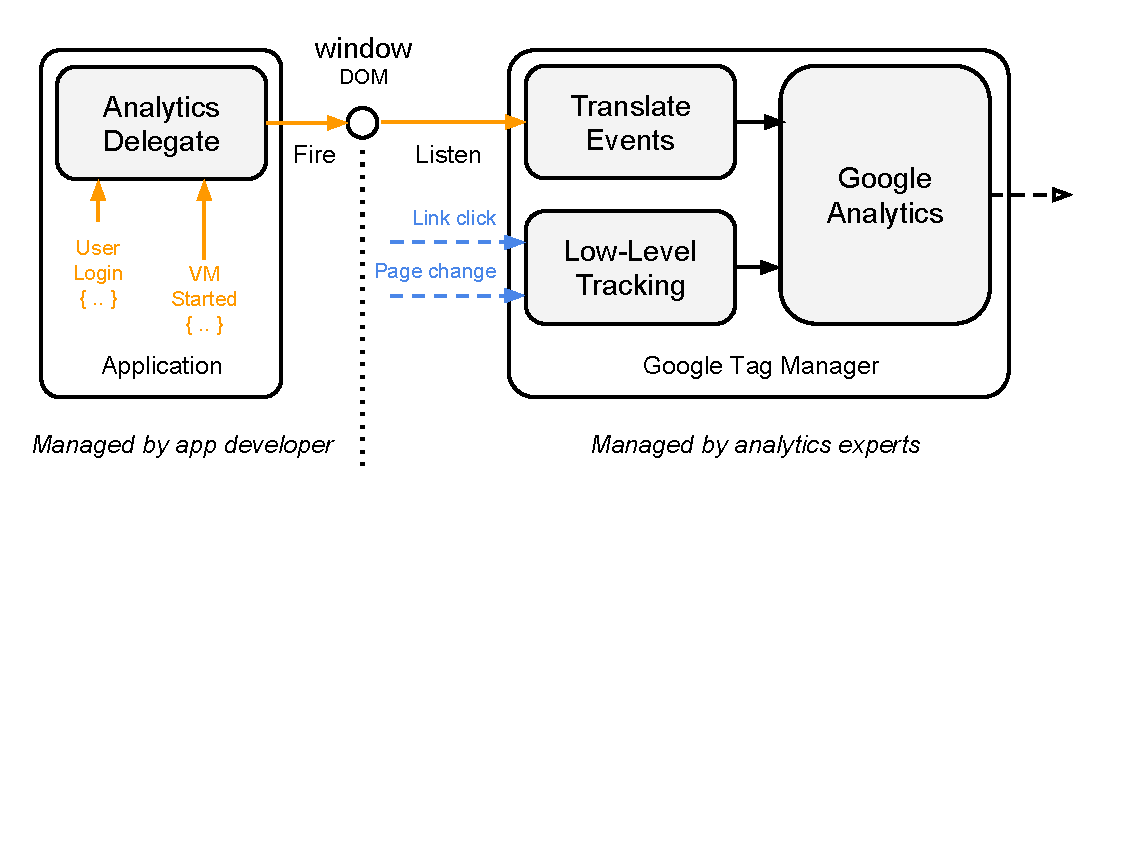
\includegraphics[width=\columnwidth]{imgs/CERN60Events.pdf}
  \end{center}
\caption{Event flow in application using CCLTracker and Google Analytics. The \CCLTrackerJS is the \emph{Analytics Delegate}, on the left}
\label{fig:cern60events}
\end{figure}

There are two different methods for fording the events to the provider: 
\begin{itemize}
\item Through a \textbf{drain function}, that will receive every event being produced, or
\item Through \textbf{event-binding} using the DOM Window as a proxy element.
\end{itemize}

The second method is favoured in our case, since the analytics logic is managed by the analytics experts and is delivered through Google Tag Manager (GTM). The developer creates a specification document describing all the events triggered by the application, and analysts use GTM to listen for particular events in the window DOM. This way, developers expose all the information required to accurately describe an event, and analysts decide to how and what is going to be processed.  

This approach is also illustrated in Figure~\ref{fig:cern60events}. The application triggers events to the \CCLTrackerJS, which get forwarded to the code provided by the analytics experts through GTM. The big benefit of this approach is the fact that additional events, that were not previously accounted for, can be tracked using the low-level tracking features of GTM or any other tracking provider.

%%%%%%%%%%%%%%%%%%%%%%%%%%%%%
\subsubsection{Persistent Store}
%%%%%%%%%%%%%%%%%%%%%%%%%%%%%

In one of our complicated examples, in the \emph{CERN 60 Computing Challenge}, it was important for us to preserve the state across browsers or sessions. That's because the user was instructed to start a Virtual Machine and we wanted to count how many hours (s)he spent on it. Our solution was to check the state of the machine every time the user comes back to the interface and if the VM is still running, accumulate the time since the last check. However, this introduced a problem, since we could not preserve the state information across different browsers.

To solve this problem, \CCLTrackerJS is equipped with a state sharing mechanism. Thus, when the state of the library is changed, a callback is fired, allowing interested parties to push the change to a persistent store. Likewise, it provides an \texttt{importStore} function for importing a previously archived state. 

In the case of CERN 60 Computing Challenge we maintained the persistent store as custom VM property, accessible through the \emph{CernVM WebAPI}~\footnote{https://github.com/wavesoft/cernvm-webapi/} library. When a browser window is focused the analytics store is restored from the VM property and when a change occurs gets immediately committed back.

%%%%%%%%%%%%%%%%%%%%%%%%%%%%%
%%%%%%%%%%%%%%%%%%%%%%%%%%%%%
\subsubsection{Usage Examples}
%%%%%%%%%%%%%%%%%%%%%%%%%%%%%
%%%%%%%%%%%%%%%%%%%%%%%%%%%%%

TODO


%
%\begin{itemize}
%\item What is CCLTracker JS library?
%\item What is the contribution of using CCLTraker library compared with starting a implementation from scratch. 
%\item Technical description of the Library
%\item Setting up the library, requirements, scope,...
%
%\end{itemize}
%

%\subsubsection{Description of the events}
%
%The tracking is implemented via high-level events fired by the Challenge interface, which are then collected and forwarded to the Google Analytics. There are two major categories of events:
%
%Related to CernVM WebAPI 
%Related to user actions
%
%The events fired to the DOM window are always prefixed with the ‘analytics.’ prefix.
%
%\subsubsection{CernVM WebAPI Events}
%
%Most of the CernVM WebAPI events are fired when the state of the internal finite-state-machine is changed. For reference, the following abstract diagram illustrates the different states in the internal FSM and the possible transitions between them:
%
%
%
%\begin{figure}[t]
%  \begin{center}
%		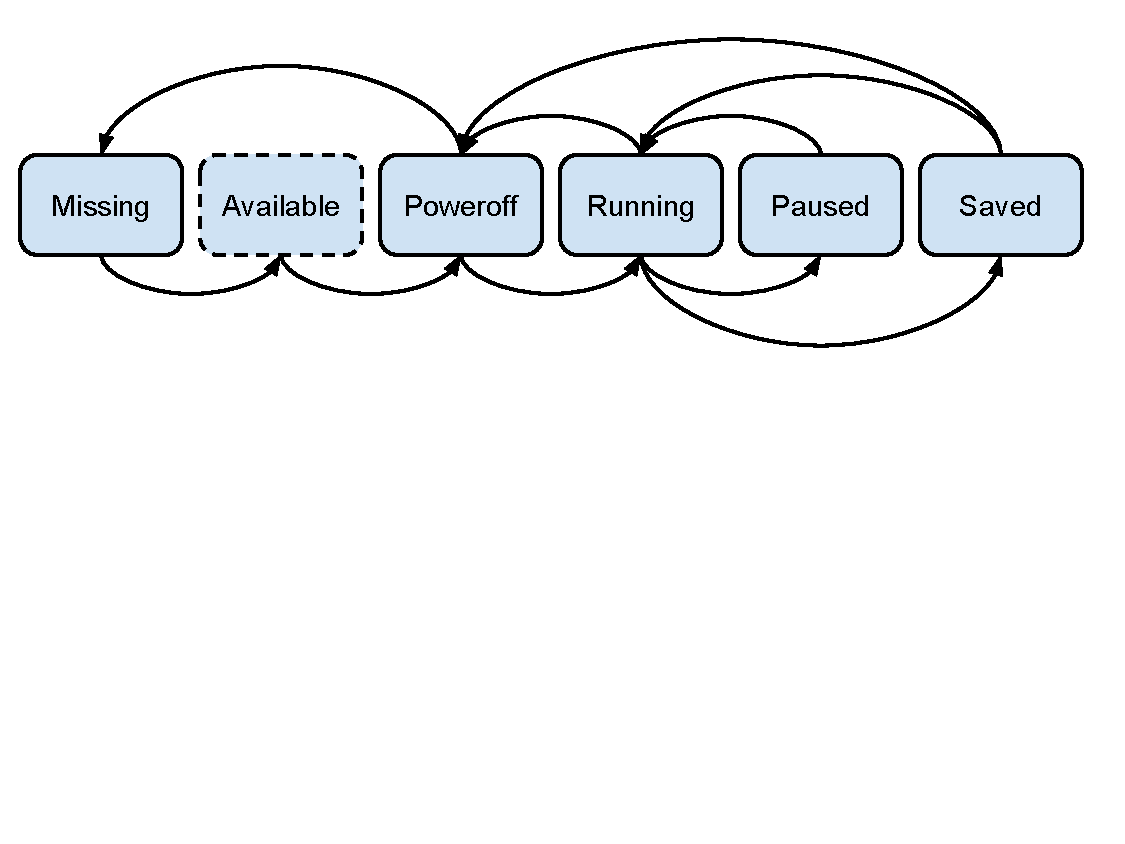
\includegraphics[width=\columnwidth]{imgs/webAPIEvents.pdf}
%  \end{center}
%\caption{xxx}
%\label{xxx}
%\end{figure}
%
%
%When the path of actions is completed and the FSM settles on a target state, the following events are fired:
%
%\begin{itemize}
%    \item {\bf vm.missing}: the VM does not exist.
%    \item {\bf vm.available}: the VM is defined in virtualbox but not yet configured.
%    \item {\bf vm.poweroff}: The VM is properly configured and powered off.
%    \item {\bf vm.saved}: the VM process has stopped and the state is saved to disk (hibernation)"
%    \item {\bf vm.paused}: the VM process is running yet it’s CPU is halted (paused in-memory).
%    \item {\bf vm.running}: the VM is running.
%\end{itemize}
%
%In addition, two special events are fired providing a higher-level information regarding the application that runs inside the Virtual Machine:
%
%\begin{itemize}
%\item {\bf vm.booted}: this event is fired when WebAPI fires the callback apiStateChanged(true), meaning that the designated port which is used for API communication between the javascript interface and the VM is available. We are assuming that the VM is “booted” because the port will be opened after the boot sequence is completed.
%
%{\textit NOTICE: This event might oscillate, because changes in the network connectivity (ex. user closing the laptop lid) will interrupt the communication, causing this event to be fired again when the network connectivity is resumed.}
%
%\item {\bf vm.collisions}: when through the API port, the javascript interface identifies that collisions are happening.
%
%{\textit NOTICE: This event has similar oscillations to vm.booted. That’s because the javascript interface is probing the job status through the API port. If the API port becomes unavailable, the interface will assume that there are no more jobs being processed. Therefore the instant it becomes available again (vm.booted), this event will be fired again.}
%
%\end{itemize}
%
%
%\subsubsection{Sequence of events}
%
%Since all these events are produced by the state changes of the FSM, they can only appear in sequences. The usual flow of events is shown on the following diagram:
%
%\begin{figure}[t]
%  \begin{center}
%		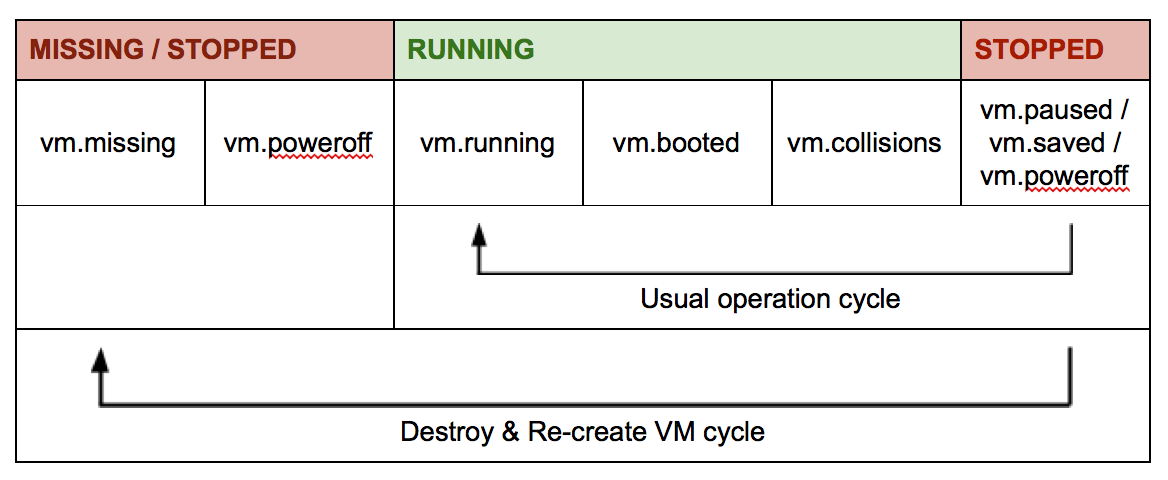
\includegraphics[width=\columnwidth]{imgs/sequenceOfEventsTable.png}
%  \end{center}
%\caption{xxx}
%\label{xxx}
%\end{figure}
%
%
%
%Therefore, you can extract some useful information:
%
%\begin{itemize}
%\item {\bf How long the VM was running?}: sum the differences in timestamps between the event "vm.running" and ANY of the following three events: "vm.paused", "vm.saved", "vm.poweroff"
%
%\item {\bf Did the user successfully manage to start a simulation?}: Check if AT LEAST one "vm.booted" event is fired after the “vm.running” event.
%\end{itemize}
%
%
%\subsubsection{User Events}
%
%These events are fired by user actions on the user interface. These are:
%
%\begin{itemize}
%    \item {\bf actions.open\_rdp}: user clicked on the "eye" icon that opens the console window. There the user can see the status of the job and the job manager.
%    
%    \item {\bf actions.open\_web}: user clicked on the "pop-out" icon that opens the website served from within the Virtual Machine. There the user can see the histograms produced by the current simulation
%actions.remove: User clicked on the trash icon which is going to remove the virtual machine from his/her computer.
%    \item {\bf actions.start}: user clicked on the “start” button, which is going to create, set-up and boot the VM. If the VM is already in any other state it will be switched to ‘running’ by following the path in the FSM diagram.
%    \item {\bf actions.stop}: user clicked on the “stop” button, which is going to SAVE the Virtual Machine to the disk (hibernate). 
%    \item {\bf actions.apply}: user clicked on the “apply” button, which is going to apply the changes (s)he did on the CPU/RAM.
%    \item {\bf actions.login}: user logged in with his/her social profile
%    \item {\bf actions.logout}: user disconnected his/her social profile
%\end{itemize}
%
%
%\subsubsection{Sequence of events with WebAPI}
%
%Most of the events fired by the WebAPI are triggered by the user. The following table shows which WebAPI events can a user event trigger. The events not included in the following table are not causing changes to the Virtual Machine.
%
%If you notice a sequence of events not matching the ones below, then the state change of the VM was most probably triggered by an external cause. 
%
%
%\begin{figure}[t]
%  \begin{center}
%		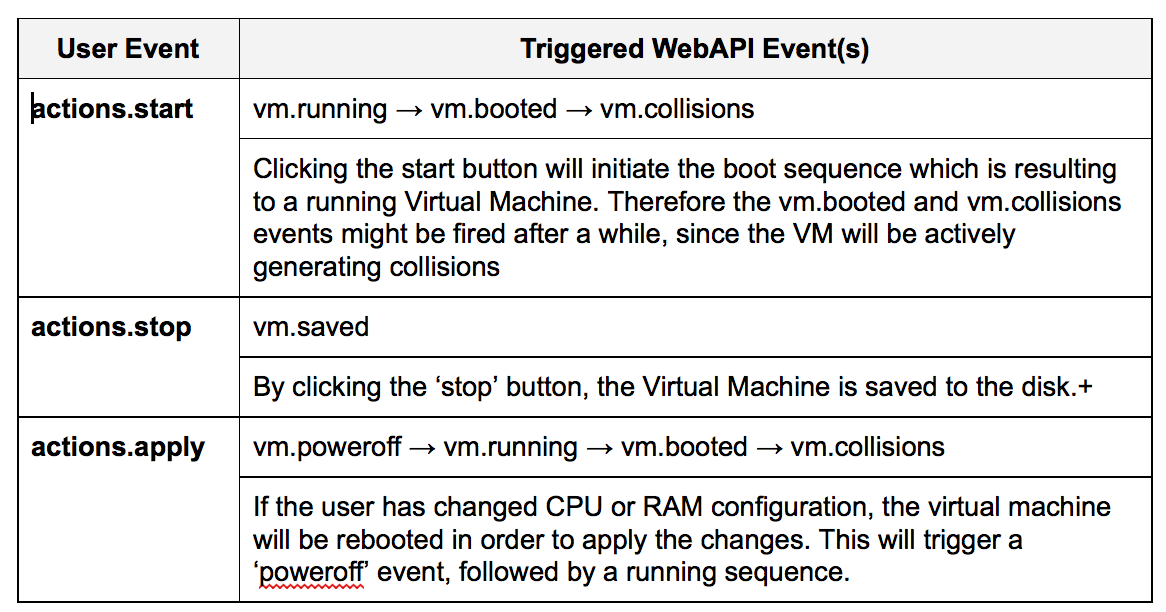
\includegraphics[width=\columnwidth]{imgs/webAPIEventsSequenceTable.png}
%  \end{center}
%\caption{xxx}
%\label{xxx}
%\end{figure}
%
%
%
%\subsubsection{Other user actions that could trigger WebAPI events}
%
%Since the user can still control the Virtual Machine without the Challenge Interface (ex. through VirtualBox), a state change can occur without a user-triggered action.
%
%
%\begin{figure}[t]
%  \begin{center}
%		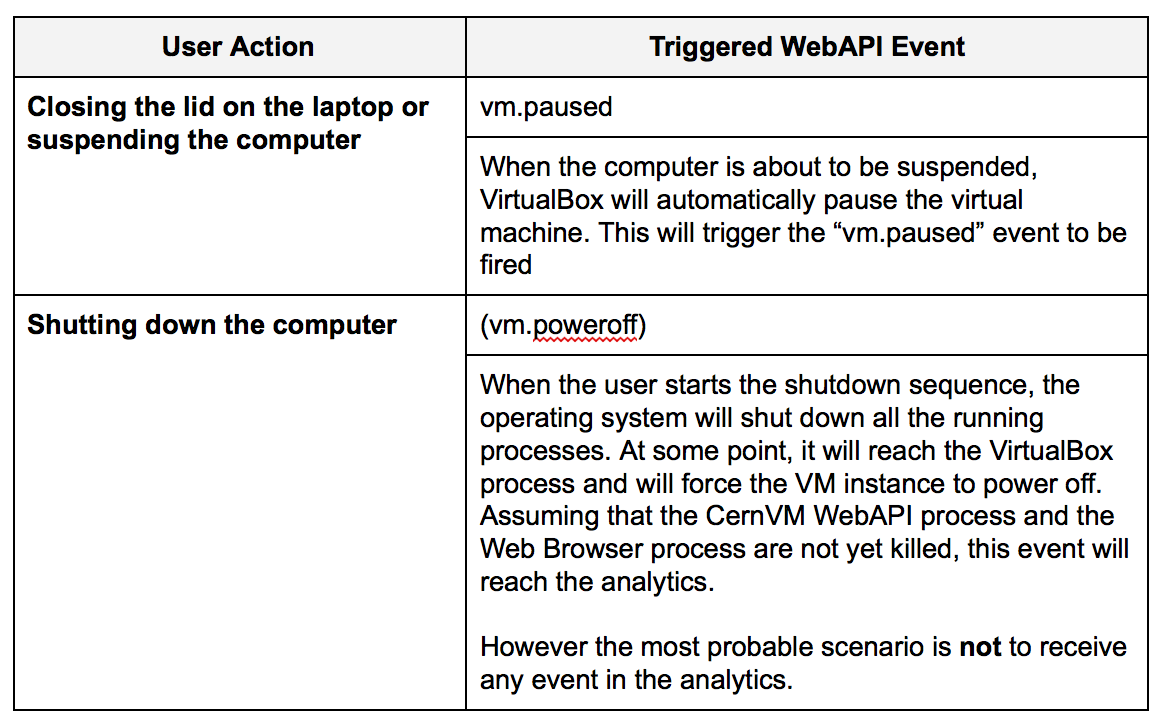
\includegraphics[width=\columnwidth]{imgs/userActions-webAPIEventsTable.png}
%  \end{center}
%\caption{xxx}
%\label{xxx}
%\end{figure}
%
%
%
%
%
%
%
%% \begin{itemize}
%% \item Briefly describe all projects using CCLtracker, Geotagx, VAS, 1st and 2nd CERN Challenges.
%% \item Focus on CERN challenges showing some examples of the data we gathered. 
%
%% \item It would be good to relate this data with the advantages we wrote in related work. 
%
%%  e.g. debugging tools --> Trace of errors combined with browsers, OS, device, etc..
%%       Knowing who are they --> Different segments and demographic information
%      
%%       Knowing their engagement --> picture about engagements. 
%      
%%       etc...
%
%% \end{itemize}
%

%%%%% 

\section{CCLTracker Framework}\label{sec:CCLtrackerFramerwork}

The CCLTracker JS Library has been integrated in a framework composed by the following tools and services:

\textbf{Google Analytics (GA)} provides storage, aggregation and visualization of data. Additionally GA provides web based analytics information. Information about users activities and system performance is sent by Google Tag Manager. 

\textbf{Google Tag Manager (GTM)} is in charge of structuring the analytics data and send it to GA. GTM receives event generated by the CCLTracker Library that are fired from the website. GTM is used as connector between the website and the analytic tool (GA in this case). By changing GTM settings we could address another analitycs tool such as Piwik, or directly store the events in a local server without requiring any change on the website code. 

\textbf{Google Query Explorer} is used to retrieve analytics data from GA. The queries created in Google Query Explorer are used in R for advance aggregation and Google Super Proxy for making data publicly available. 

\textbf{R language} is used to created advance aggregation of analytics data. It allows us to measure engagement in many different ways, and using cluster algorithms for gather users profiles. 

\textbf{Google Super Proxy} allows us to make public analytics data, and share it with the website users. 


One of the major decisions taken in this framework was the use of GA. GA was adapted as analytics tools because the demographics information they provide, the fast set up time, it is a free service, and its strong community using it. 



\begin{figure}[t]
  \begin{center}
		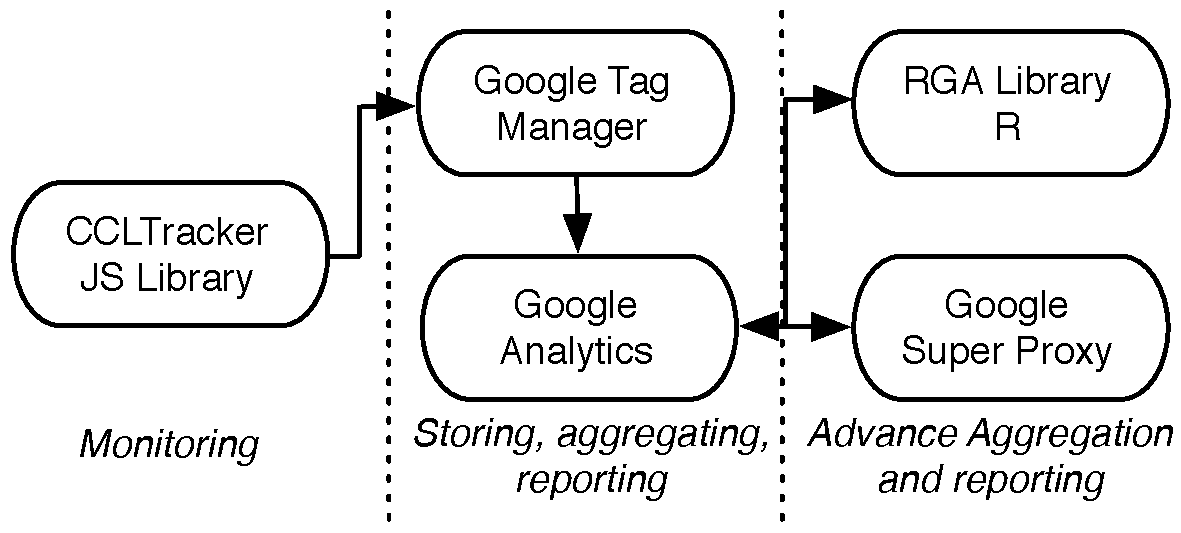
\includegraphics[width=11cm]{imgs/ccltrackerFramework.pdf}
  \end{center}
\caption{CCLTracker Framework Components}
\label{img:CCLTrackerFrameworkComponents}
\end{figure}

Figure~\ref{img:CCLTrackerFrameworkComponents} shows the interaction between the different components of the CCLTracker Framework. 


% Notice that there is not a dependency between the CCLTracker Library and GA. Events generated by the CCLTracker Library can be received from Google Tag Manager and sent to GA, or it can be received from GTM and send to Piwik, or it could be received from an external process and store the data in a local data base. 


\section{Proof of concept}

This section summarises the main applications where the CCLTracker framework has been used and show data examples. 

The CCLTracker framework has been implemented under the EU project Citizen CyberLab. The main goal was to evaluate the different pilots developed during the project, evaluate the engagement, dissemination actions, and evaluate users learning outcomes.

CCLTracker framework has been implemented in the following pilots:

\begin{itemize}
\item \textbf{CERN Volunteer Computing Challenge}\footnote{https://test4theory.cern.ch/challenge/} is  web site running periodic public volunteer computing challenges. Volunteers help CERN scientists simulate particle collisions in accelerators like the Large Hadron Collider (LHC), using their own computers. 

\item \textbf{GeoTag-X}\footnote{www.geotagx.org/} is a website focuses on crowdsource photo analysis for humanitarian disaster response.

\item \textbf{Virtual Atom Smasher}\footnote{http://test4theory.cern.ch/about/} is an educational interactive game that teaches users about particle physics, while in the same time helps theoretical physicists at CERN with their research.
\end{itemize}


The CCLTracker Framework has been integrated in these applications in order to understand the users behaviour, measuring engagement and users' learning. 


\subsection{CERN Volunteer Computing Challenges}

CERN volunteer computing challenges is a periodic volunteer computing event. The CCLTracker framework has been used in two of those events. Namely, at the CERN 60 Challenges, 12-days event that run during the last days of December 2014 (9-20 Dec.), and the CERN Public Computing Challenge 2015 that run from 1st Nov to 1st Dic 2015. The purpose of these challenges were to test the experimental CernVM WebAPI technology and to understand users behaviour and interest behind volunteer computing project. Analytics information gathered from CCLTracker is used for measuring engagement, evaluate the user interface and for evaluating the CERN VM Technology. 


\begin{figure}[th]
  \begin{center}
		\includegraphics[width=11cm]{imgs/challenge.png}
  \end{center}
\caption{CERN Public Computing Challenge 2015)}
\label{img:challenge}
\end{figure}


Basically, the events monitored by the CCLTracker framework are clissified into 3 groups:

\textbf{Users actions} contains all events related with user actions on the challenge website such as clicking external links, start button,  stop button, or changing the  virtual machine settings (i.e. number of cores and memory the user is donating). 

\textbf{Users goals}: are used to monitor user achievements over the participation on the challenge. Some examples are CPU time donated, number of jobs computed, or how many times an user starts the VM. Goals are pre-aggregated before firing the event. This has two main advantages: (1) it easy the data analysis and (2) it allows to extract demographic data for different user segments based on participation (e.g. gender of users who has contribute more than 100 jobs, or interest of user who visit the website but did not contribute). 

\textbf{VM status}: contains all event related with the status of the virtual machine such as available, paused, running, stopped, or booted. Additionally, all erros are also reported as events. Reporting errors allows us to debug the application without waiting for user feedback. When combined with Google analytics, errors can be crossed with browsers, OS, mobile or desktop device information. Thus, making easier to find and reproduce error and finally to improve the quality of the software. 

\textbf{WebAPIStatus}:contains events related with the web interface to the Virtual Machine.



\subsection{GeoTag-X}

Geotag-X is a pilot project within Citizen Cyberlab to develop and test tools to engage and educate volunteers in analysing photos coming out of humanitarian crises, with the aim of producing datasets that can be used in relief and recovery efforts by disaster response agencies.



\begin{figure}[th]
  \begin{center}
		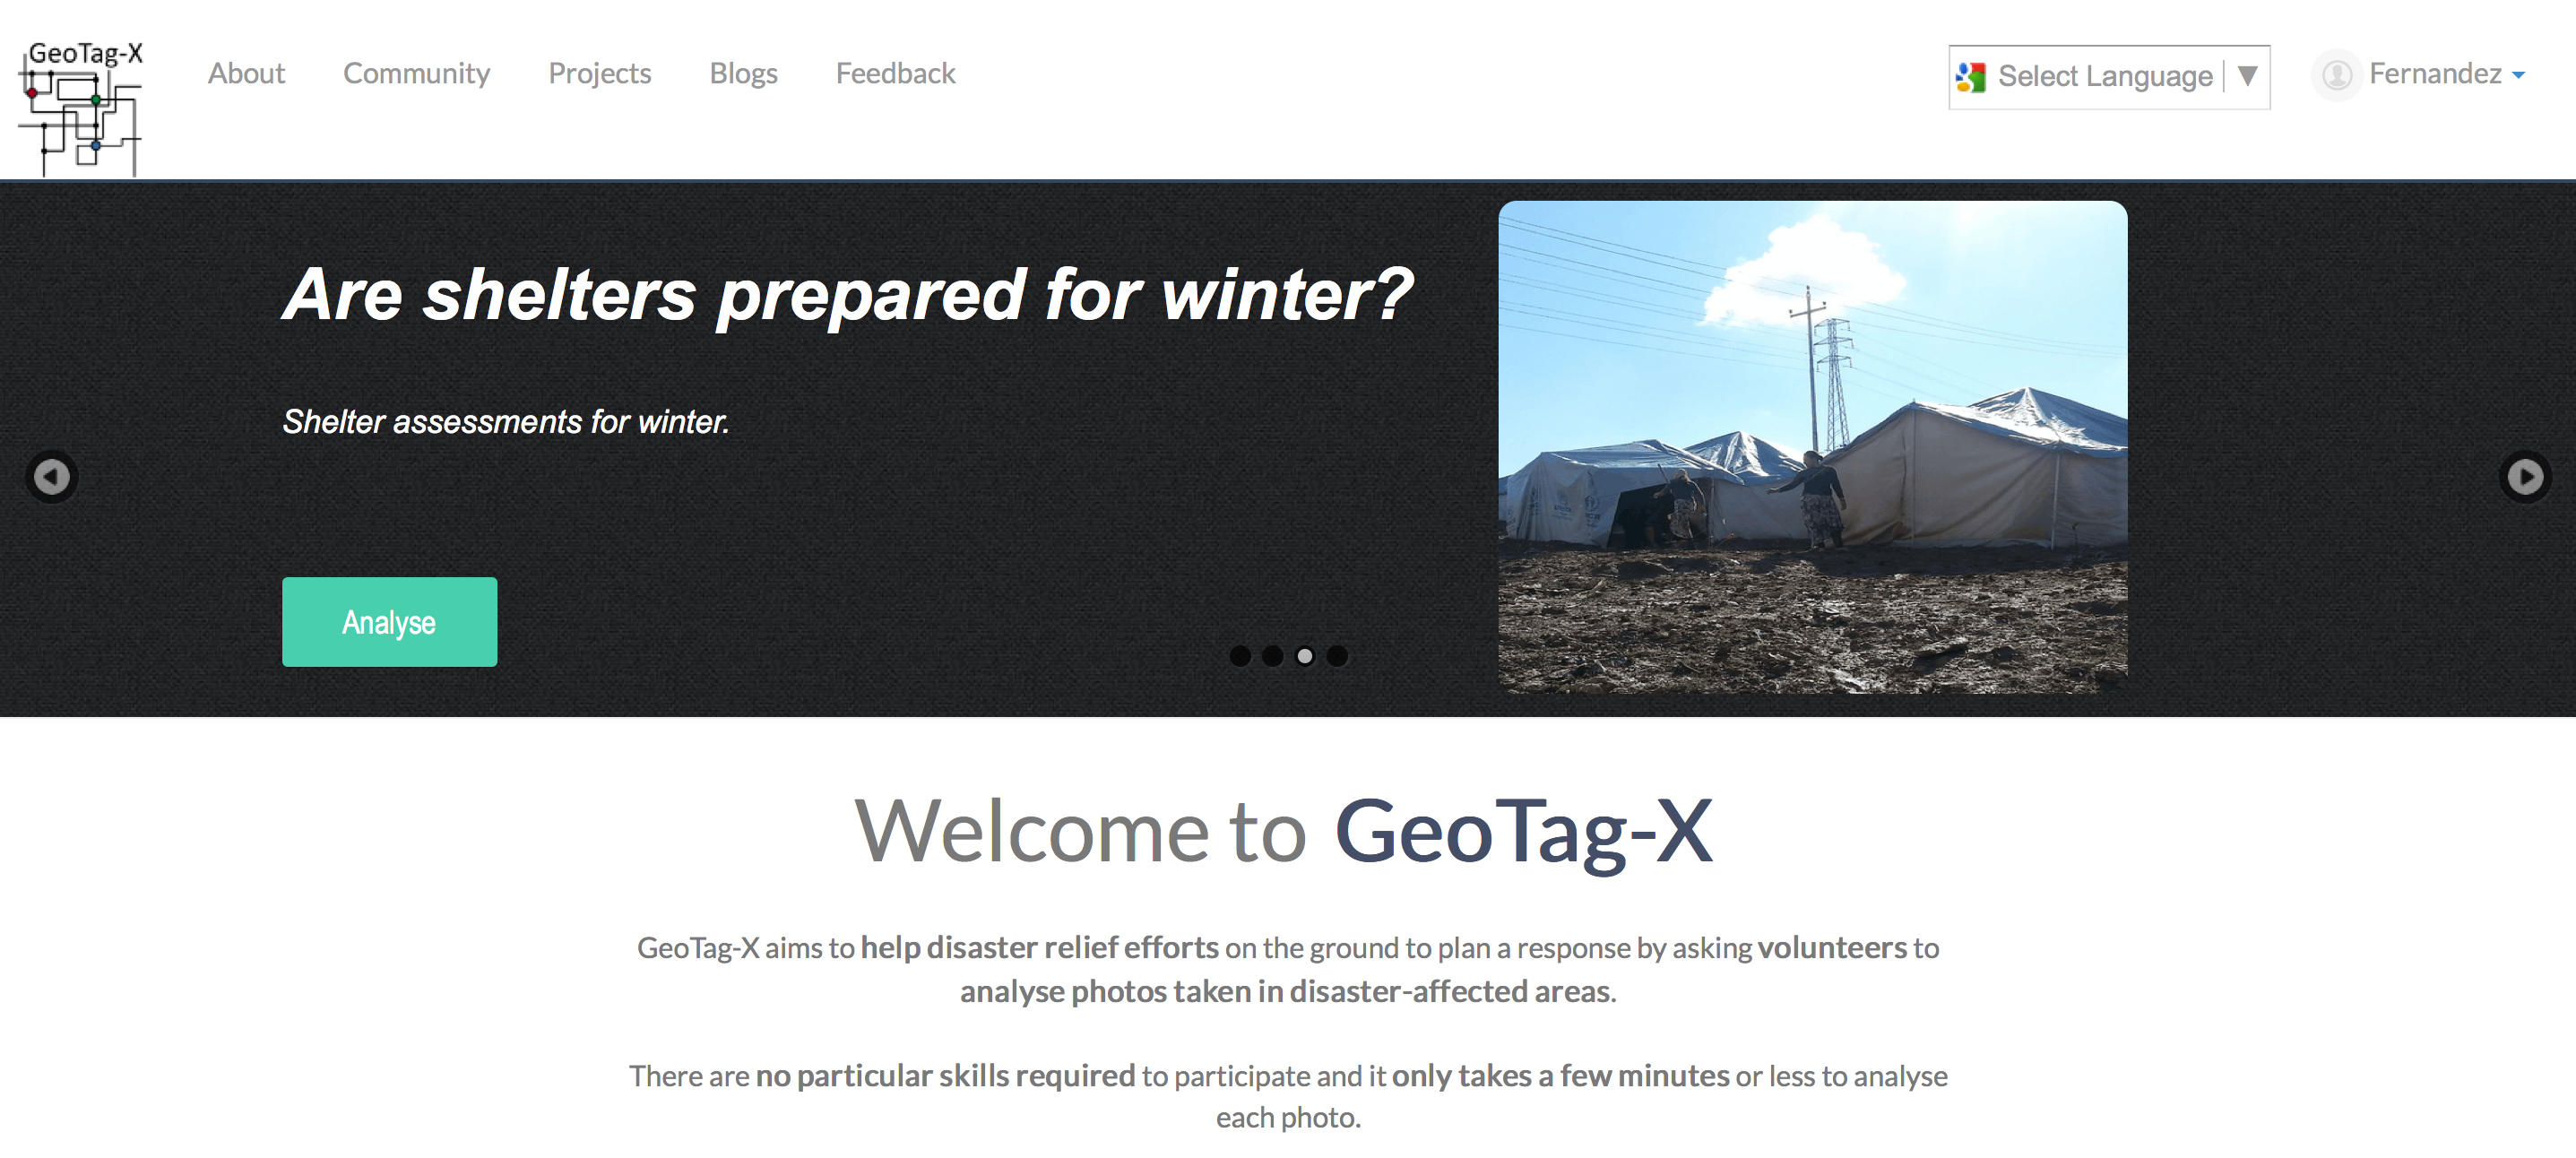
\includegraphics[width=11cm]{imgs/geotagx.png}
  \end{center}
\caption{GeoTag-X application}
\label{img:geotagx}
\end{figure}


\subsection{VAS Game}

Virtual Atom Smasher is an educational game that	allows citizens	to contribute to scientific discoveries at	CERN without any prior knowledge	of particle physics. They	control a Monte Carlo event generator (a virtual	particle collider) that produces scientific	data	analogous to the ones generated by the real High Energy Physics experiments, and their goal is to tune its parameters until the results match the measured	experimental results. The outcomes are important to the scientific community, since they can validate the current scientific hypotheses.

\begin{figure}[th]
  \begin{center}
		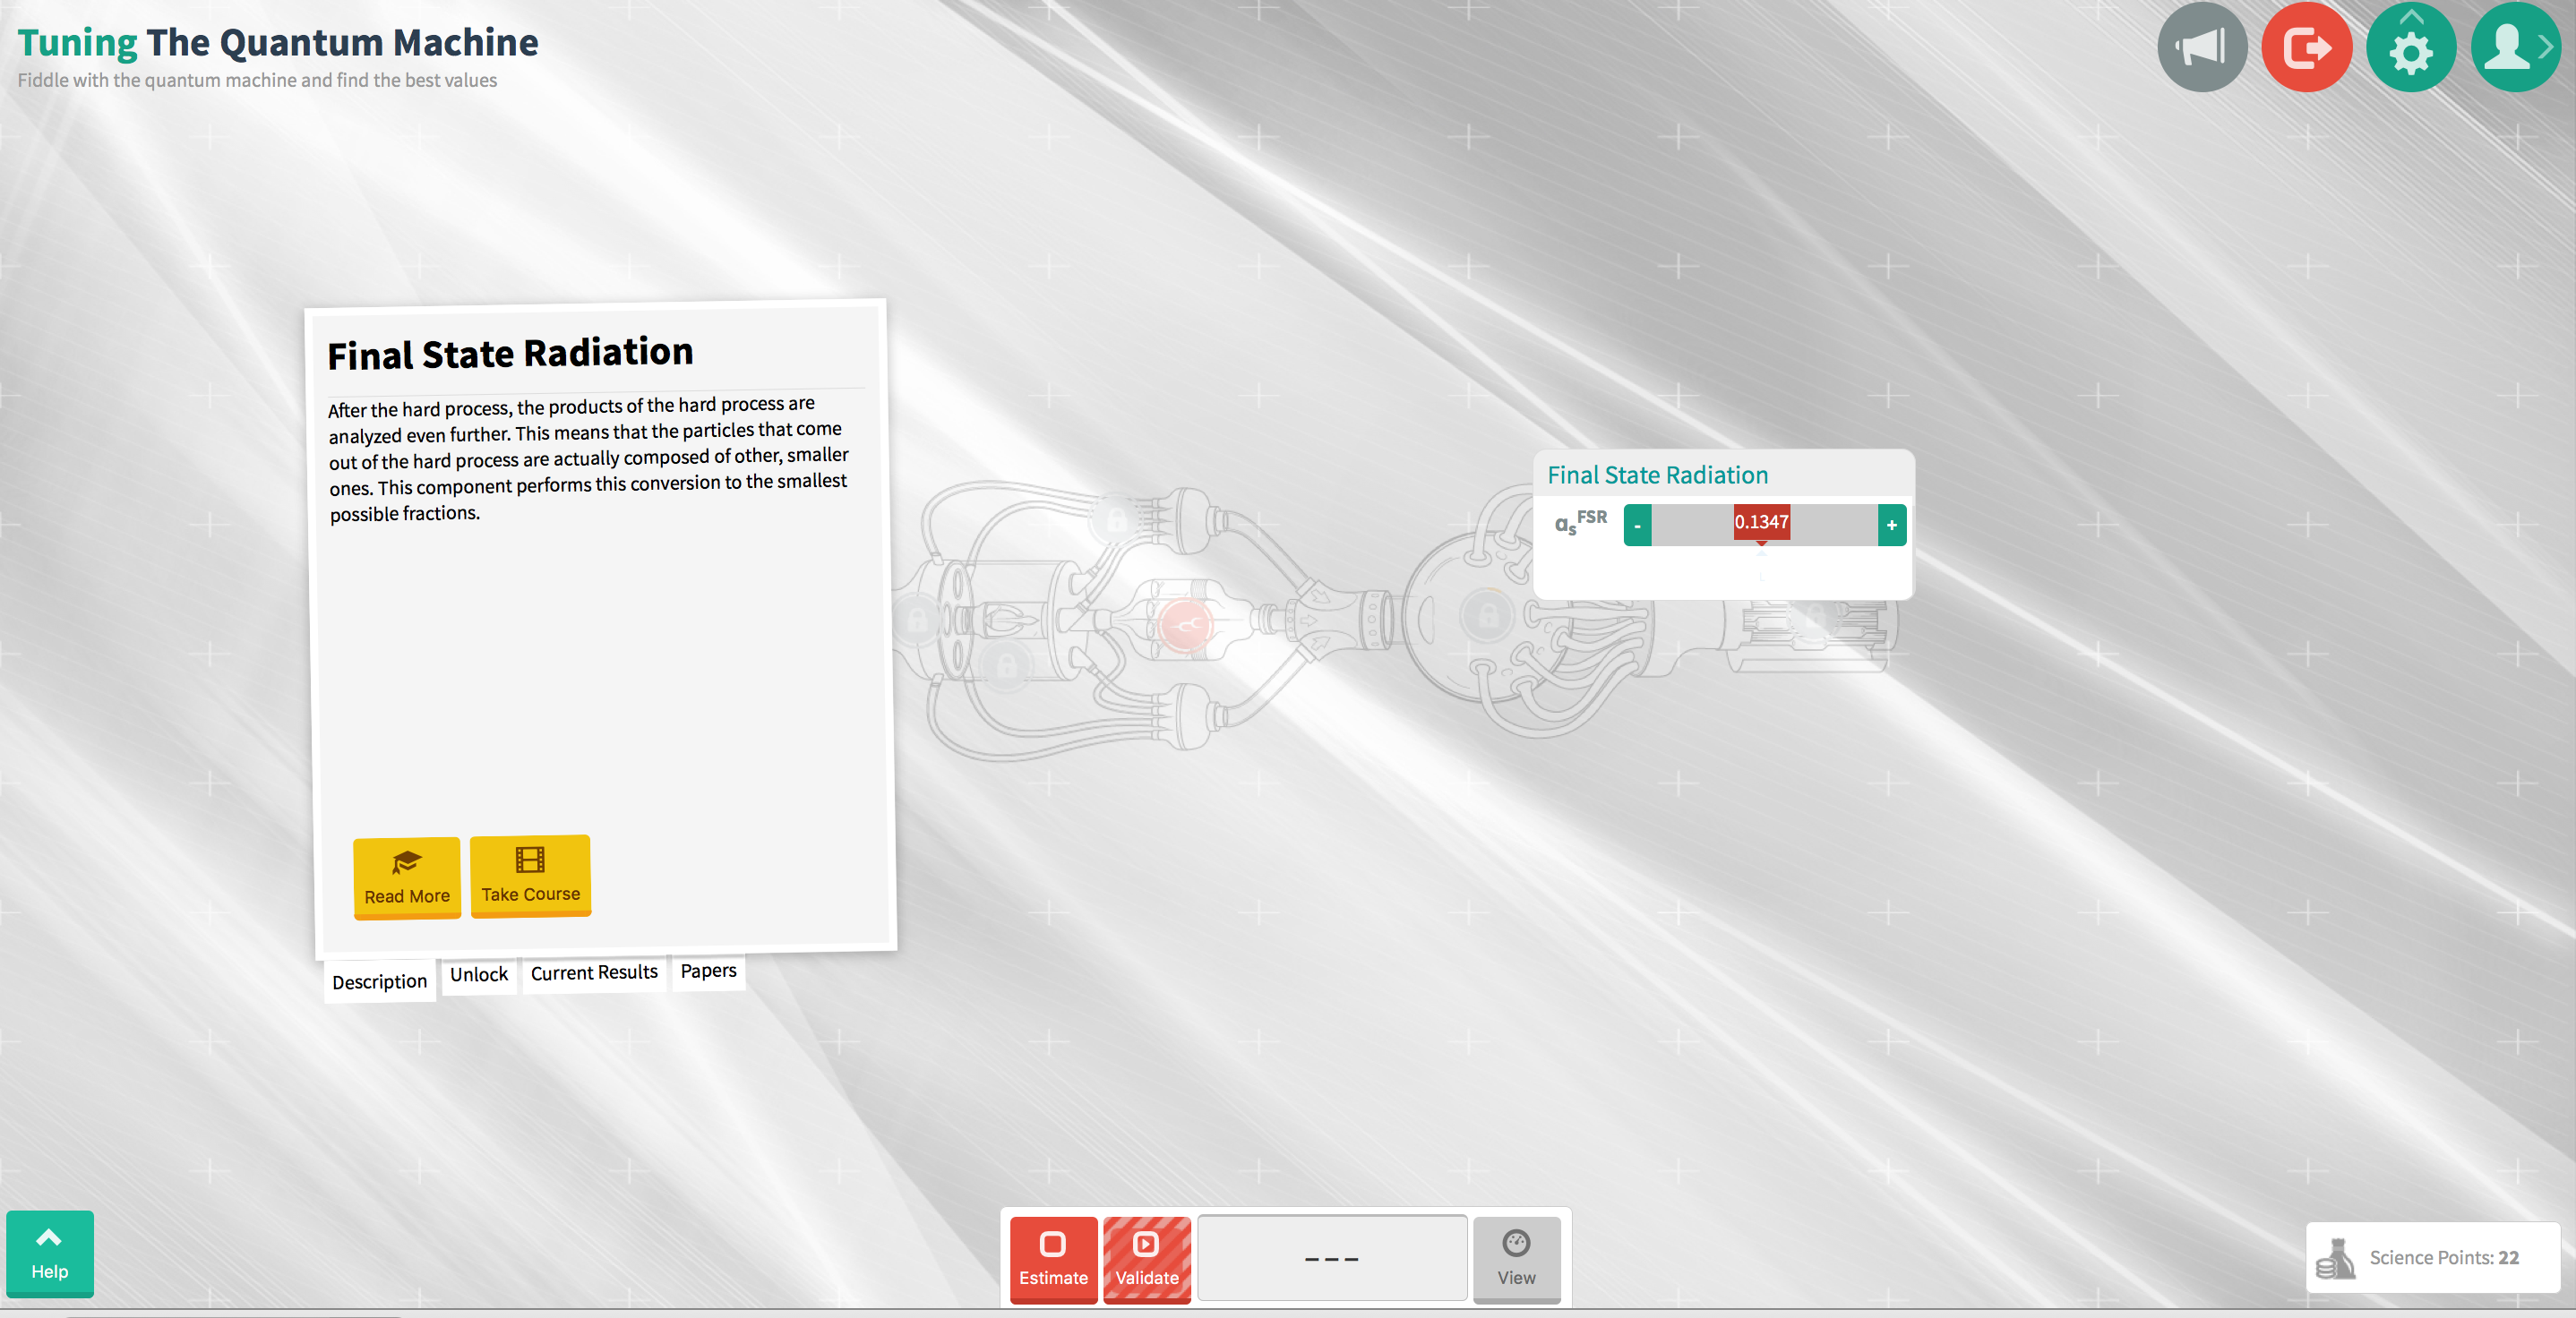
\includegraphics[width=11cm]{imgs/vas.png}
  \end{center}
\caption{Virtual Atome Smasher game}
\label{img:vas}
\end{figure}



%\subsubsection{Event forwarding specifications}
%
%We are using Google Analytics for handing the analytics events, which is delivered through Google Tag Manager. The latter offers the ability to dynamically inject additional tracking logic at a later time. However due to the complexity of the processes involved, it’s frequently not easy to identify the events of interest from an external library. For instance, it might be easy to track clicks on the “Start” button, but it’s not easy to understand if this action really started the Virtual Machine.
%
%Therefore we need to have a higher-level information that should come directly from the application. In order to accommodate future changes in the way the analytics data are processed, we agreed on an interface between the application developer and the analytics experts. 
%
%
%\begin{figure}[t]
%  \begin{center}
%		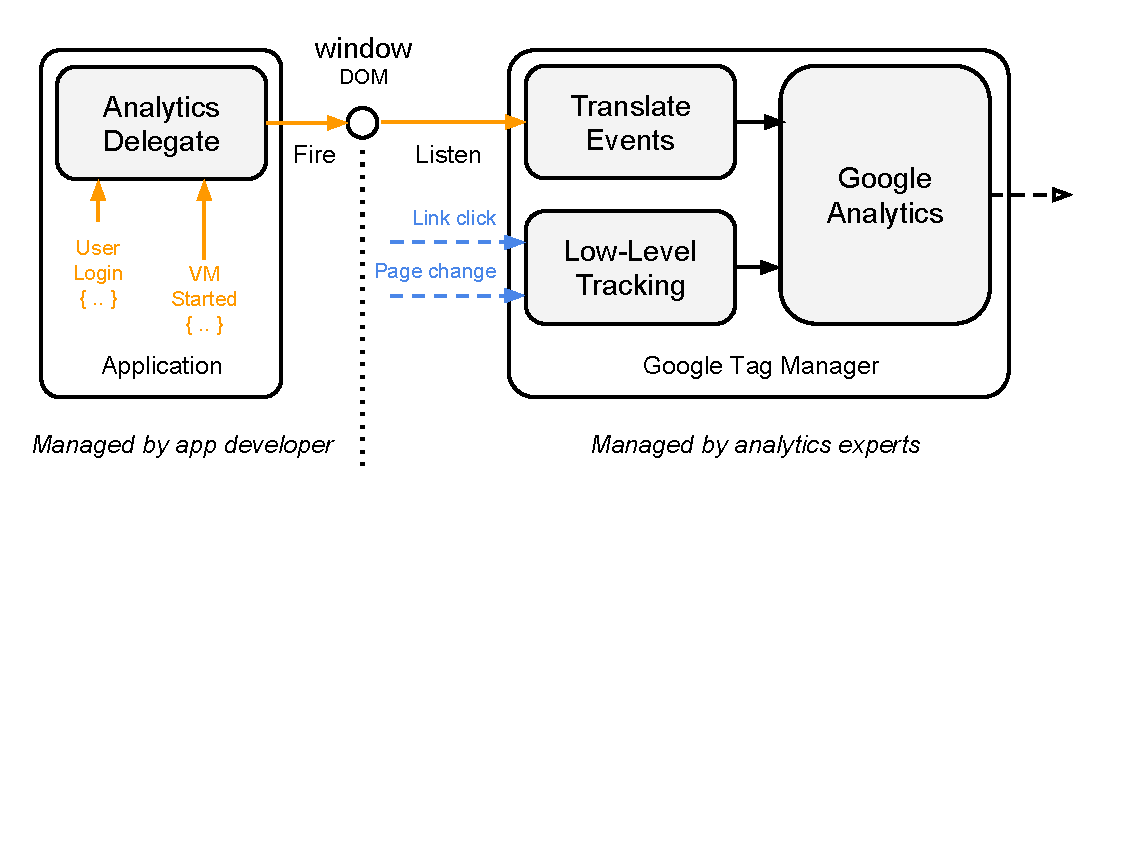
\includegraphics[width=\columnwidth]{imgs/CERN60Events.pdf}
%  \end{center}
%\caption{xxx}
%\label{xxx}
%\end{figure}
%
%
%
%As seen in the above diagram, the application developer is triggering high-level events to an Analytics Delegate class. This class is then firing the appropriate events to the window DOM, not requiring anyone to listen for them.
%
%When the analytics logic is managed by the analytics experts and is delivered via Google Tag Manager. It listens for analytics events in the window DOM, translates them to an appropriate format and forwards them to Google Analytics. The developer and the analytics experts maintain a document that lists all the possible events fired by the Analytics Delegate, along with the information each event carries. This way, they can optimally select and/or pre-process the high-level events into their preferred format.
%
%In addition, the analytics experts can deliver extra, low-level tracking logic (for example listening for mouse clicks or page changes) that can provide them with additional information as required.
%
%\subsubsection{Description of the events}
%
%The tracking is implemented via high-level events fired by the Challenge interface, which are then collected and forwarded to the Google Analytics. There are two major categories of events:
%
%Related to CernVM WebAPI 
%Related to user actions
%
%The events fired to the DOM window are always prefixed with the ‘analytics.’ prefix.
%
%\subsubsection{CernVM WebAPI Events}
%
%Most of the CernVM WebAPI events are fired when the state of the internal finite-state-machine is changed. For reference, the following abstract diagram illustrates the different states in the internal FSM and the possible transitions between them:
%
%
%
%\begin{figure}[t]
%  \begin{center}
%		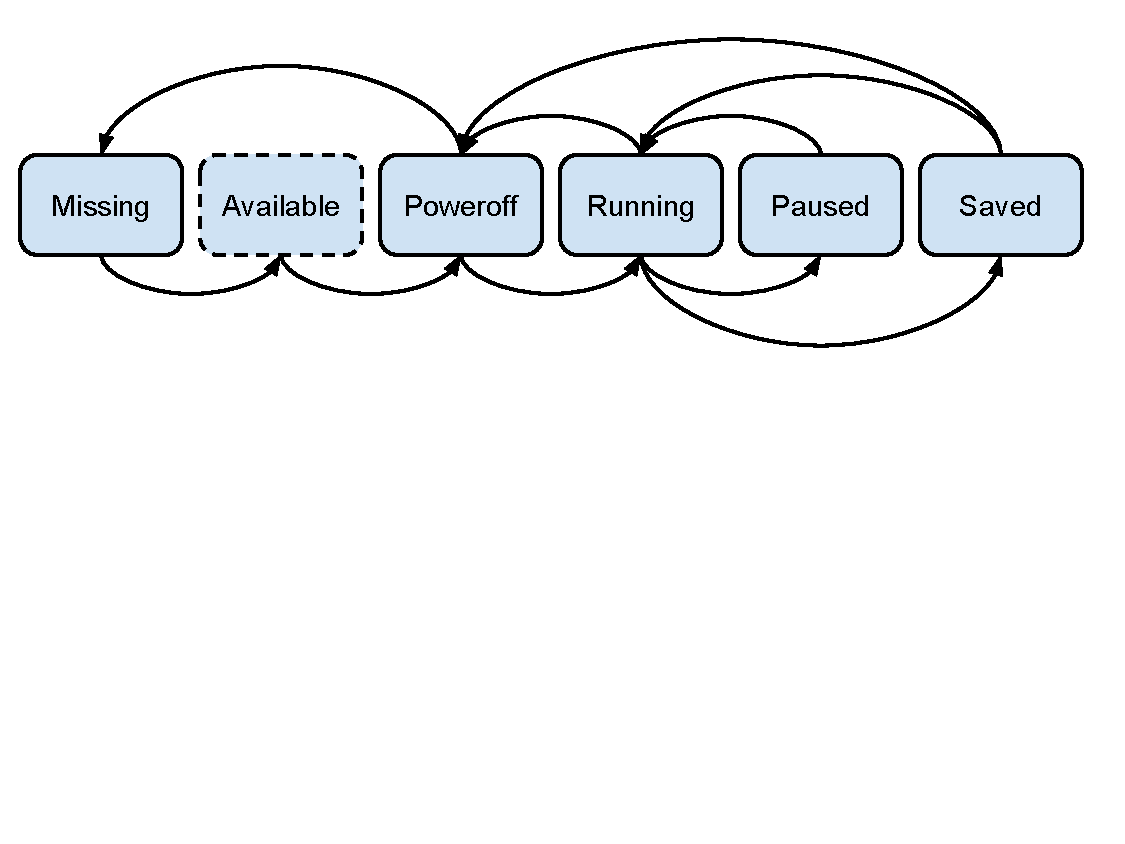
\includegraphics[width=\columnwidth]{imgs/webAPIEvents.pdf}
%  \end{center}
%\caption{xxx}
%\label{xxx}
%\end{figure}
%
%
%When the path of actions is completed and the FSM settles on a target state, the following events are fired:
%
%\begin{itemize}
%    \item {\bf vm.missing}: the VM does not exist.
%    \item {\bf vm.available}: the VM is defined in virtualbox but not yet configured.
%    \item {\bf vm.poweroff}: The VM is properly configured and powered off.
%    \item {\bf vm.saved}: the VM process has stopped and the state is saved to disk (hibernation)"
%    \item {\bf vm.paused}: the VM process is running yet it’s CPU is halted (paused in-memory).
%    \item {\bf vm.running}: the VM is running.
%\end{itemize}
%
%In addition, two special events are fired providing a higher-level information regarding the application that runs inside the Virtual Machine:
%
%\begin{itemize}
%\item {\bf vm.booted}: this event is fired when WebAPI fires the callback apiStateChanged(true), meaning that the designated port which is used for API communication between the javascript interface and the VM is available. We are assuming that the VM is “booted” because the port will be opened after the boot sequence is completed.
%
%{\textit NOTICE: This event might oscillate, because changes in the network connectivity (ex. user closing the laptop lid) will interrupt the communication, causing this event to be fired again when the network connectivity is resumed.}
%
%\item {\bf vm.collisions}: when through the API port, the javascript interface identifies that collisions are happening.
%
%{\textit NOTICE: This event has similar oscillations to vm.booted. That’s because the javascript interface is probing the job status through the API port. If the API port becomes unavailable, the interface will assume that there are no more jobs being processed. Therefore the instant it becomes available again (vm.booted), this event will be fired again.}
%
%\end{itemize}
%
%
%\subsubsection{Sequence of events}
%
%Since all these events are produced by the state changes of the FSM, they can only appear in sequences. The usual flow of events is shown on the following diagram:
%
%\begin{figure}[t]
%  \begin{center}
%		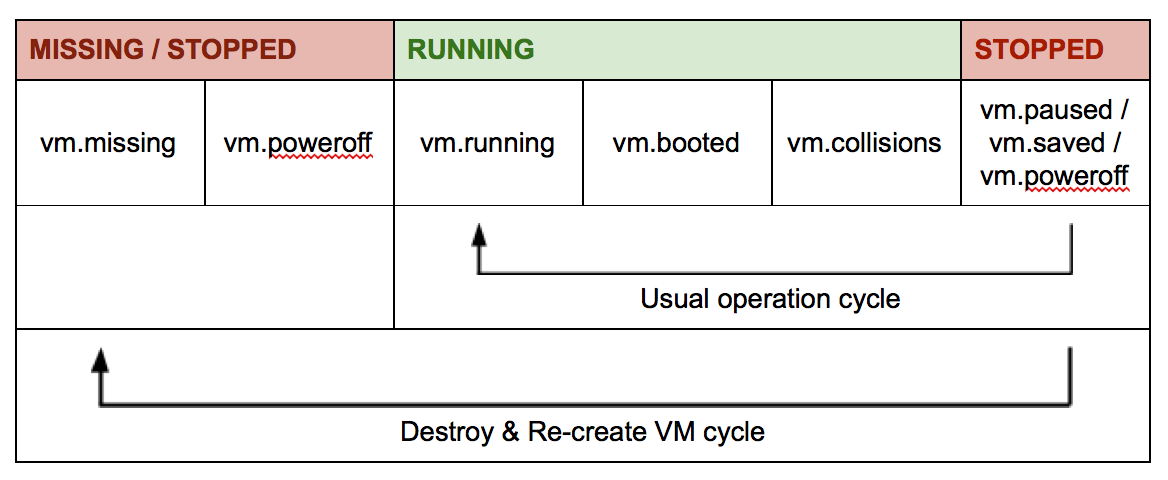
\includegraphics[width=\columnwidth]{imgs/sequenceOfEventsTable.png}
%  \end{center}
%\caption{xxx}
%\label{xxx}
%\end{figure}
%
%
%
%Therefore, you can extract some useful information:
%
%\begin{itemize}
%\item {\bf How long the VM was running?}: sum the differences in timestamps between the event "vm.running" and ANY of the following three events: "vm.paused", "vm.saved", "vm.poweroff"
%
%\item {\bf Did the user successfully manage to start a simulation?}: Check if AT LEAST one "vm.booted" event is fired after the “vm.running” event.
%\end{itemize}
%
%
%\subsubsection{User Events}
%
%These events are fired by user actions on the user interface. These are:
%
%\begin{itemize}
%    \item {\bf actions.open\_rdp}: user clicked on the "eye" icon that opens the console window. There the user can see the status of the job and the job manager.
%    
%    \item {\bf actions.open\_web}: user clicked on the "pop-out" icon that opens the website served from within the Virtual Machine. There the user can see the histograms produced by the current simulation
%actions.remove: User clicked on the trash icon which is going to remove the virtual machine from his/her computer.
%    \item {\bf actions.start}: user clicked on the “start” button, which is going to create, set-up and boot the VM. If the VM is already in any other state it will be switched to ‘running’ by following the path in the FSM diagram.
%    \item {\bf actions.stop}: user clicked on the “stop” button, which is going to SAVE the Virtual Machine to the disk (hibernate). 
%    \item {\bf actions.apply}: user clicked on the “apply” button, which is going to apply the changes (s)he did on the CPU/RAM.
%    \item {\bf actions.login}: user logged in with his/her social profile
%    \item {\bf actions.logout}: user disconnected his/her social profile
%\end{itemize}
%
%
%\subsubsection{Sequence of events with WebAPI}
%
%Most of the events fired by the WebAPI are triggered by the user. The following table shows which WebAPI events can a user event trigger. The events not included in the following table are not causing changes to the Virtual Machine.
%
%If you notice a sequence of events not matching the ones below, then the state change of the VM was most probably triggered by an external cause. 
%
%
%\begin{figure}[t]
%  \begin{center}
%		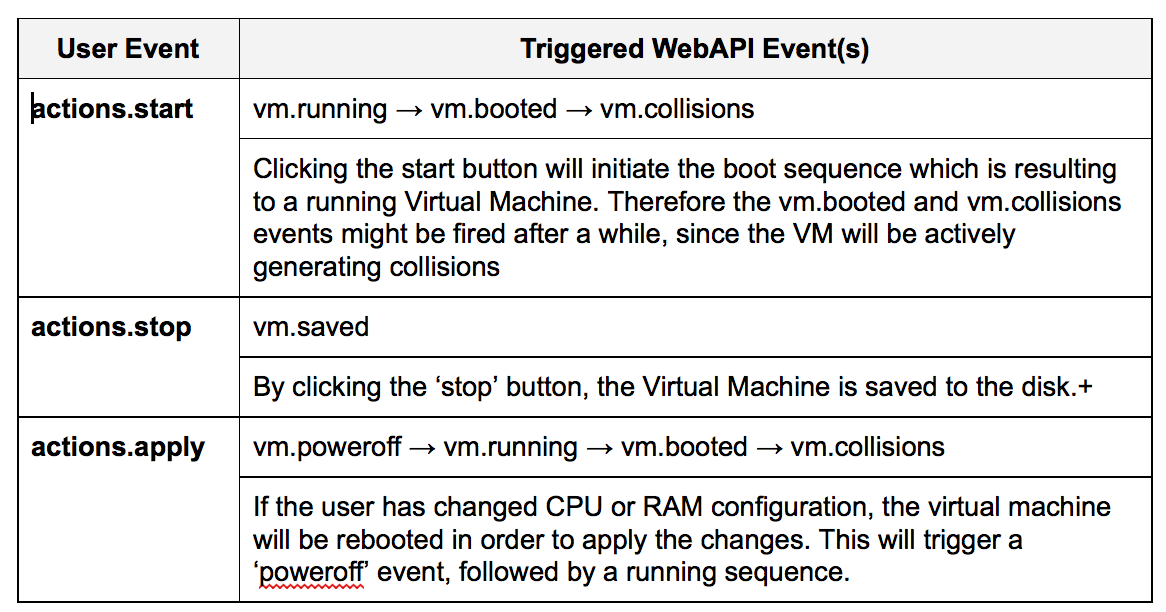
\includegraphics[width=\columnwidth]{imgs/webAPIEventsSequenceTable.png}
%  \end{center}
%\caption{xxx}
%\label{xxx}
%\end{figure}
%
%
%
%\subsubsection{Other user actions that could trigger WebAPI events}
%
%Since the user can still control the Virtual Machine without the Challenge Interface (ex. through VirtualBox), a state change can occur without a user-triggered action.
%
%
%\begin{figure}[t]
%  \begin{center}
%		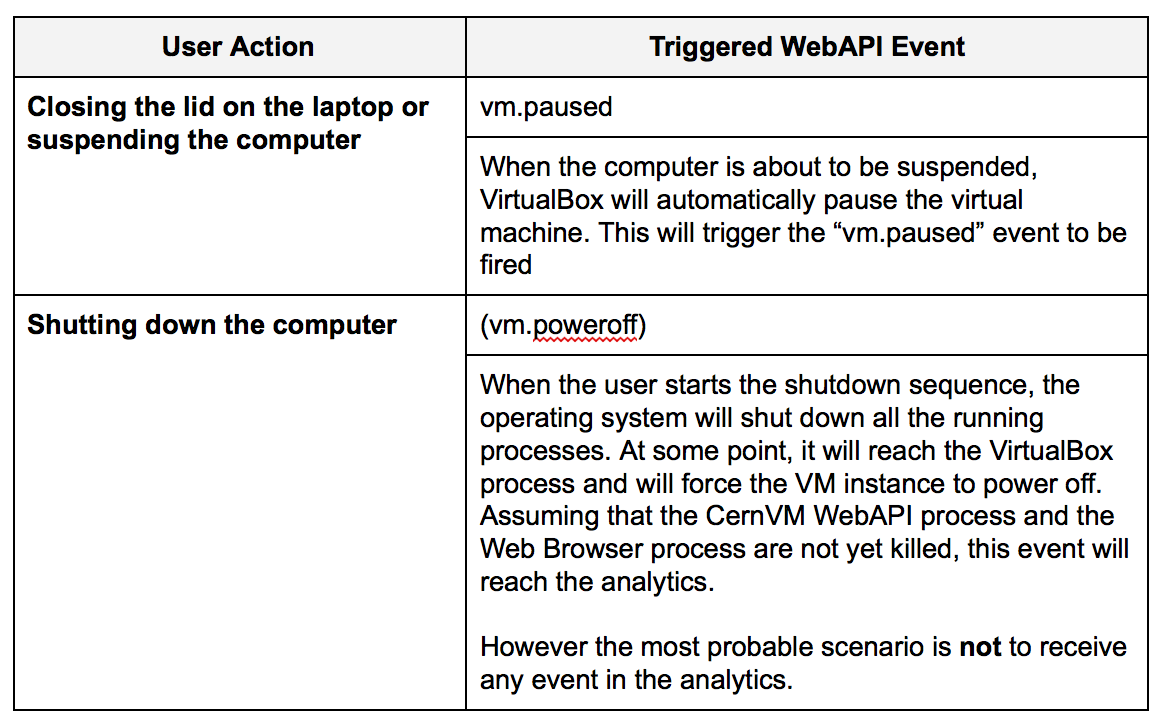
\includegraphics[width=\columnwidth]{imgs/userActions-webAPIEventsTable.png}
%  \end{center}
%\caption{xxx}
%\label{xxx}
%\end{figure}
%
%
%
%
%
%
%
%% \begin{itemize}
%% \item Briefly describe all projects using CCLtracker, Geotagx, VAS, 1st and 2nd CERN Challenges.
%% \item Focus on CERN challenges showing some examples of the data we gathered. 
%
%% \item It would be good to relate this data with the advantages we wrote in related work. 
%
%%  e.g. debugging tools --> Trace of errors combined with browsers, OS, device, etc..
%%       Knowing who are they --> Different segments and demographic information
%      
%%       Knowing their engagement --> picture about engagements. 
%      
%%       etc...
%
%% \end{itemize}
%




\subsection{Data analysis}



This section shows results gathered from the CERN Volunteer Computing Challenges, GeoTag-X and VAS using the CCLTracker framework. 

\subsubsection{CERN volunteer computing challenges}

CCLTracker allows us to measure the participation based on contribution to the citizen science projects. In this case we can distiguis between visitors (i.e. users who visit the site but they do not contribute on the challenge) and participant (i.e. those users who install the virtual machine and share computational resources). 

Figure \ref{img:visitorsVSparticipants} shows the number of visitors and participants, and their number of sessions. One of the key ingredient to measuring learning outcomes and engagement is to monitor user participation. 



\begin{figure}[t]
	\begin{center}
		\subfigure[]{
			   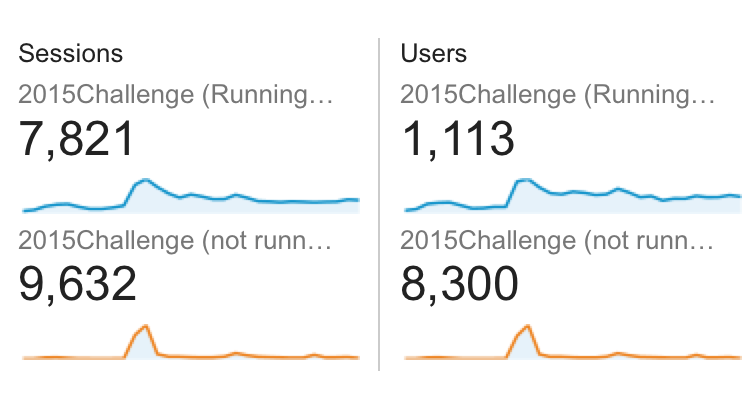
\includegraphics[width=0.50\columnwidth]{imgs/RunningVSNoRunningVM(sessionsandusers).png}
		}
		\subfigure[]{
	 		  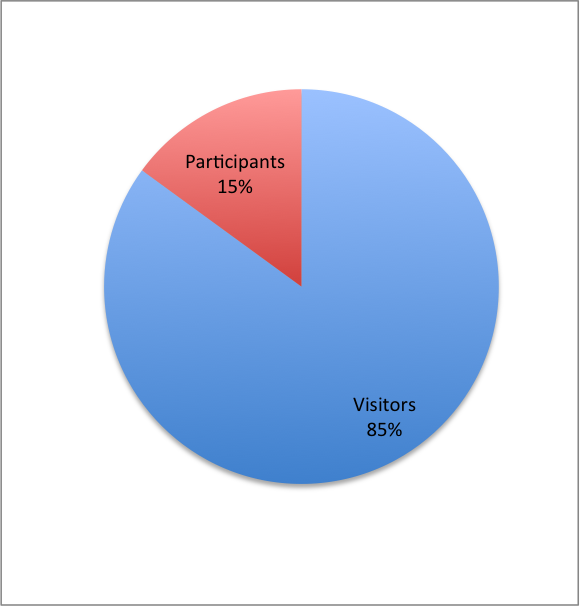
\includegraphics[width=0.34\columnwidth]{imgs/VisitorVSParticipants-Percentage.png}
		 }
		 \subfigure[]{
			   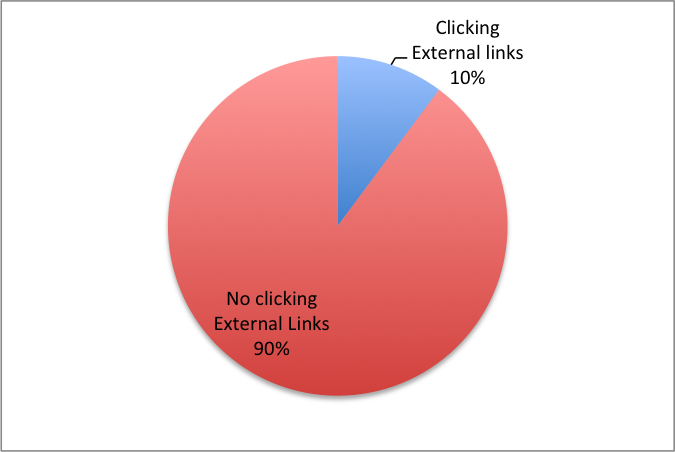
\includegraphics[width=0.45\columnwidth]{imgs/externalLinks.png}
		 }
	\end{center}
	\caption{Challenge participation  (a) Visitors/participants, (b) \% participants and visitors, and (c) user clicking external links}
	\label{img:visitorsVSparticipants}
\end{figure} 





Figure \ref{img:SessionsVSsessions running the VM} shows the number of sessions per day coming from visitors and participants. Blue line represents visitors and orange represents  participant. We could appreciate the peaks generated by different dissemination actions, and the percentage of participants engaged from the actions. In this way we can measured the impact of dissemination actions beyond the number of visitors, i.e. how many real participants are we gathering for each dissemination action.  


\begin{figure*}[th]
  \begin{center}
		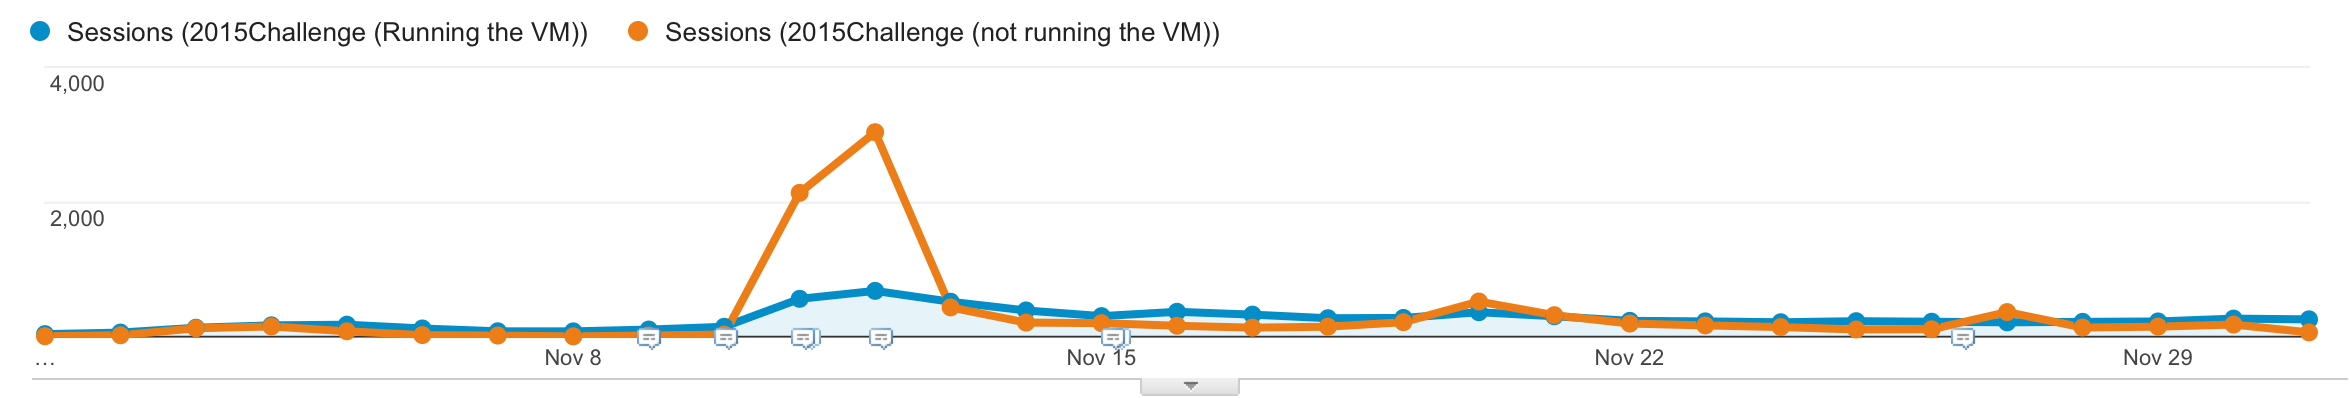
\includegraphics[width=15cm]{imgs/sessionVSsessionVMRunning.png}
  \end{center}
\caption{Sessions of users not running the VM versus sessions running the VM}
\label{img:SessionsVSsessions running the VM}
\end{figure*}



We established different levels of participation in order to measure the user engagement and get web based analytics information such as referrals, demographic information, or interest for the different participation levels. Figure \ref{img:usersbyjobs} shows the number of users for the different participation levels, i.e. at least 1 job, 5 jobs, 10 jobs, etc...



\begin{figure}[t]
  \begin{center}
		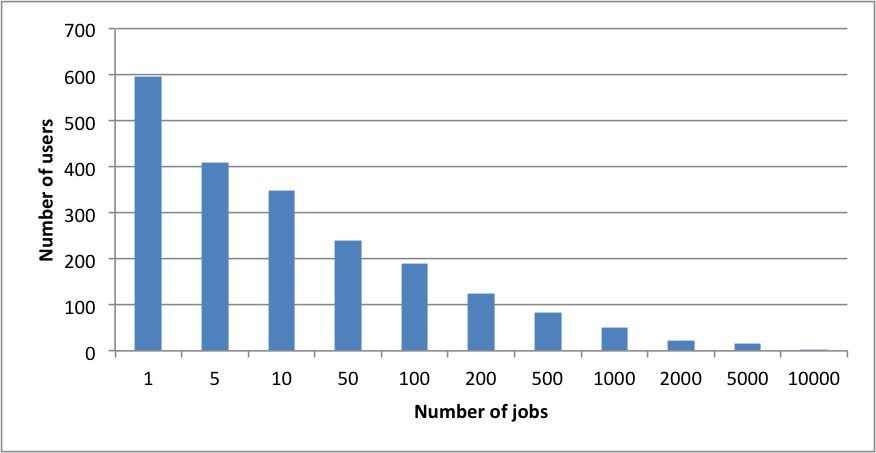
\includegraphics[width=11cm]{imgs/usersbyjobs.png}
  \end{center}
\caption{Number of users by level of participation (number of jobs processed)}
\label{img:usersbyjobs}
\end{figure}


The number of jobs computed could be subject to the computational resources of the user machine. Thus, the level of participation could be computed also by the CPU time donated to the event. Figure \ref{img:usersbycputime} shows the number of users for each participation level based on the hours the CPU processing data from the challenge. 

\begin{figure}[t]
  \begin{center}
		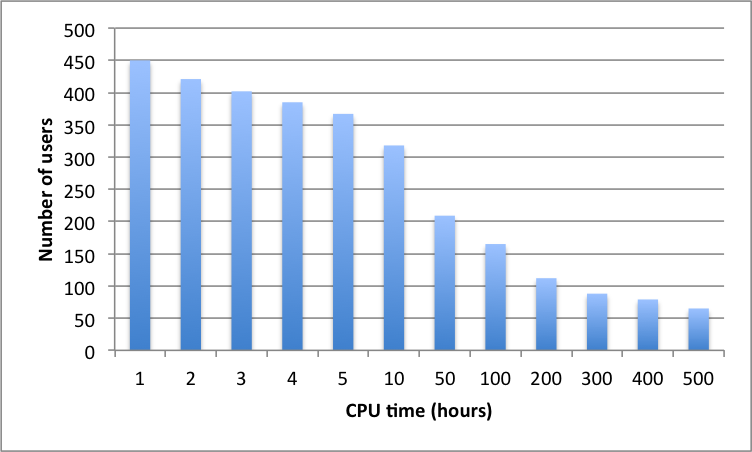
\includegraphics[width=11cm]{imgs/usersbycputime.png}
  \end{center}
\caption{Number of users by level of participation (CPU time donated)}
\label{img:usersbycputime}
\end{figure}



CCLTracker framework also allows to cross user location with participation information, thus we can see the participation form each county and the participation level of the user coming from each country (see Figure \ref{img:Participationbycountry}).



\begin{figure}[t]
  \begin{center}
		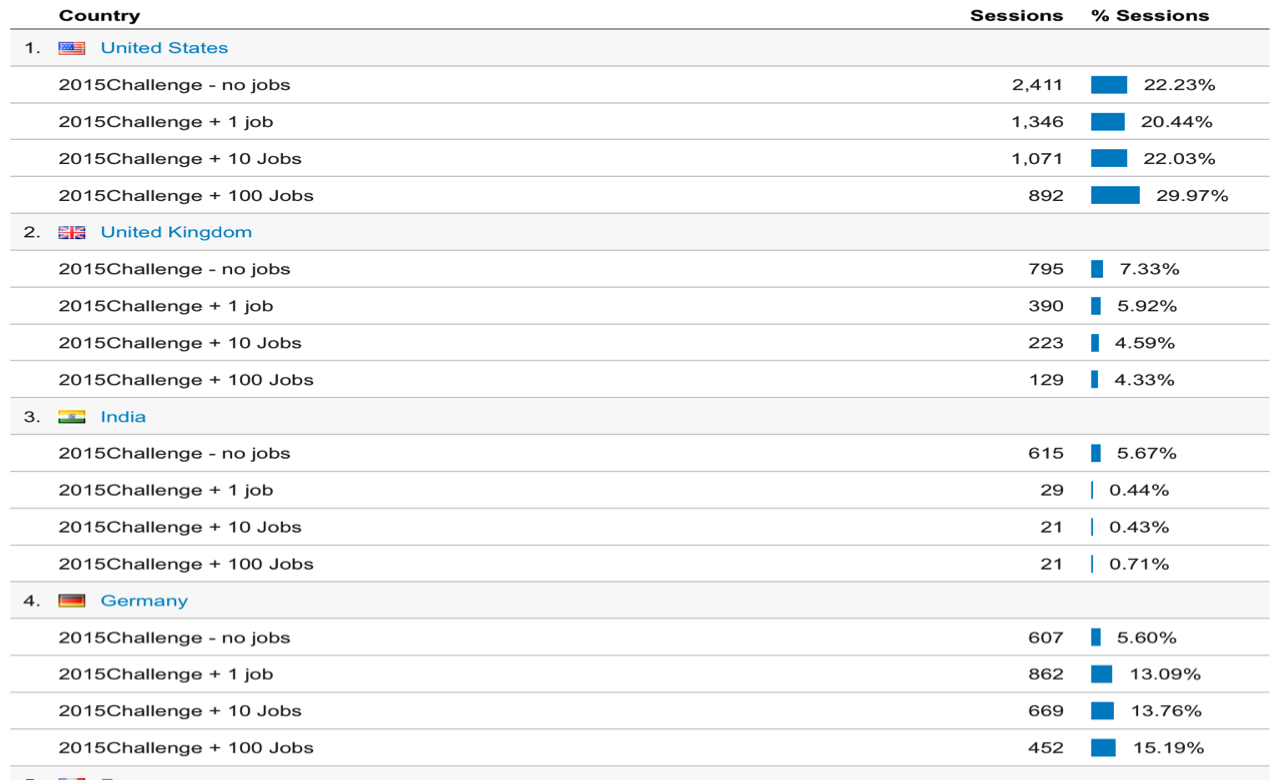
\includegraphics[width=11cm]{imgs/participationByCountry.png}
  \end{center}
\caption{Participation by countries}
\label{img:Participationbycountry}
\end{figure}


Additionally, we can evaluate the users participation coming from the different referrals (see Figure \ref{img:usersbyreferrals} ). This is specially relevant to measure dissemination actions and emproving user engagement.


\begin{figure}[t]
  \begin{center}
		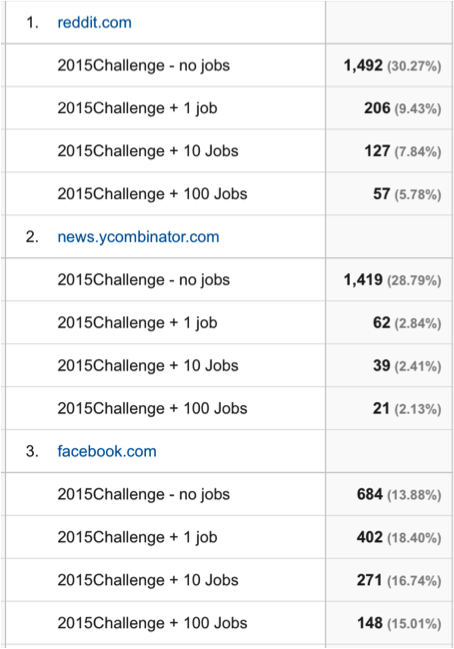
\includegraphics[width=7cm]{imgs/usersbyreferrals.png}
  \end{center}
\caption{Number of Participants by referrals}
\label{img:usersbyreferrals}
\end{figure}



CCLTracker allows to combine demographic information from Google analytics with monitoring information coming from CCLTracker JS library. In this case we can see the evolution of gender balance for different levels of participation. Figure\ref{img:genderchallenge} shows the gender balance for users who do not compute any job, at least one job,  more than 10 jobs and finally more than 100 jobs. Notice that 1 job requires around 1 to 2 hours depending on the computational power of the machine and the percentage donated to the event. Visitors, i.e. users not contributing any job can easily be changed by addressing specific communities on the dissemination actions. However, high active users like those one computing more than 100 jobs represent the profile of the volunteer computing community. I.e. we can address female users by addressing association for women in sciences or teenagers by addressing high schools. That ensures to increase the number of women and teenages as visitors, but it do not ensure that they will high contribute on the project. 


\begin{figure}[t]
	\begin{center}
		\subfigure[no jobs]{
		   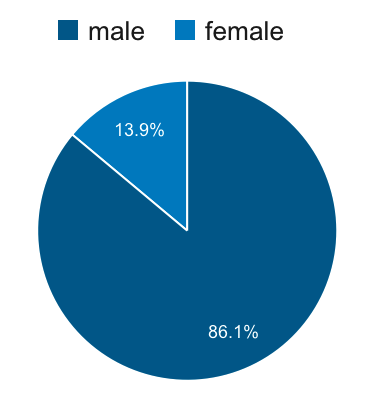
\includegraphics[width=0.36\columnwidth]{imgs/gender-nojobs.png}
		 }
	\subfigure[at least 1 job]{
 		  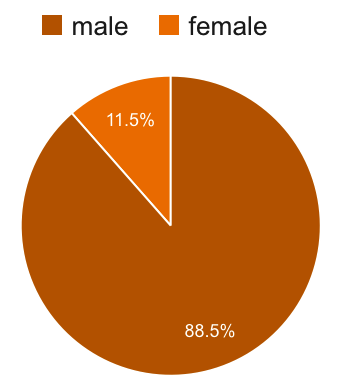
\includegraphics[width=0.34\columnwidth]{imgs/gender-1job.png}
	 }
	 \subfigure[more than 10 jobs]{
		   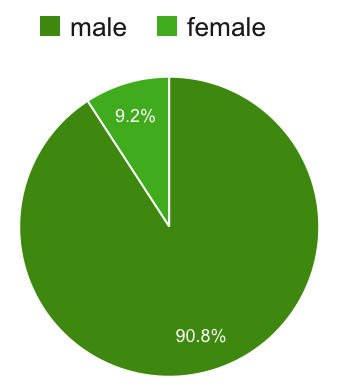
\includegraphics[width=0.34\columnwidth]{imgs/gender-10jobs.png}
	 }
	 \subfigure[more than 100 jobs]{
		   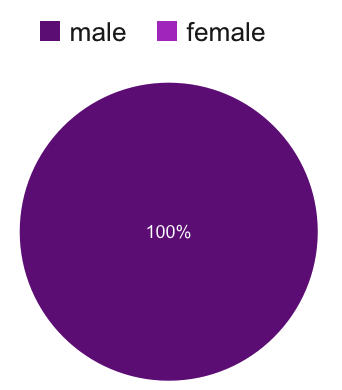
\includegraphics[width=0.34\columnwidth]{imgs/gender-100jobs.png}
	 }
	\end{center}
	\caption{Users' gender balance  (a) users not computing any job, (b) users computing at least 1 jobs, (c) users computing more than 10 jobs, and (d) users computing more than 100 jobs}
	\label{img:genderchallenge}
\end{figure} 
      
    
    
    
%      
%      
%\begin{figure}[t]
%  \begin{center}
%		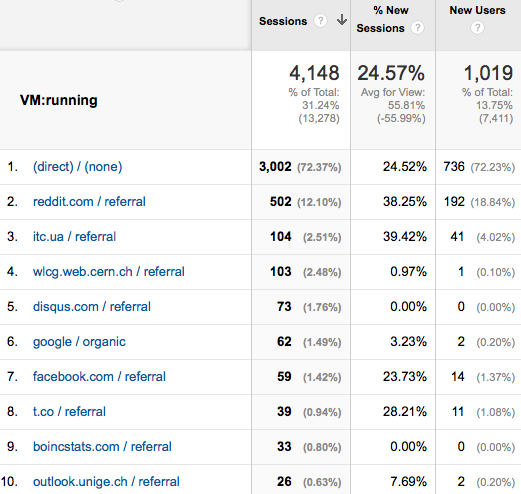
\includegraphics[width=\columnwidth]{imgs/sourceMediumVMRunning.png}
%  \end{center}
%\caption{Acquisition - Num. of sessions running VM by Source/Medium}
%\label{img:AcquisitionRunningVM}
%\end{figure}      
%      
%      
%
%
%\begin{figure}[t]
%  \begin{center}
%		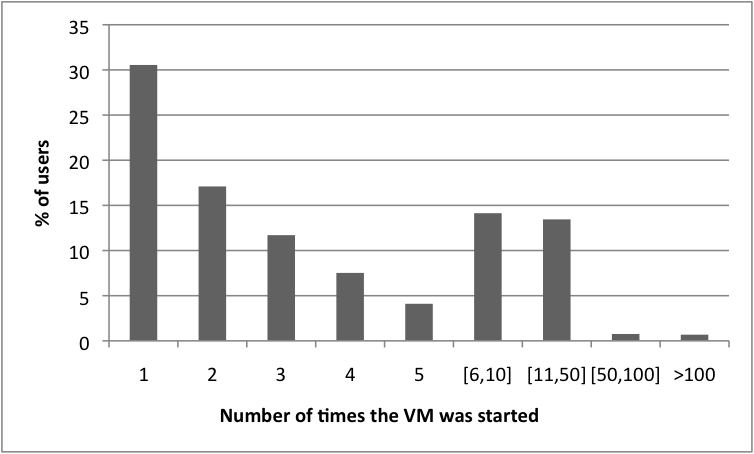
\includegraphics[width=\columnwidth]{imgs/Engagement.png}
%  \end{center}
%\caption{Engagement - number of times users are running the VM}
%\label{img:EngagementVMrunning}
%\end{figure}
%
%
%\begin{figure}[t]
%  \begin{center}
%		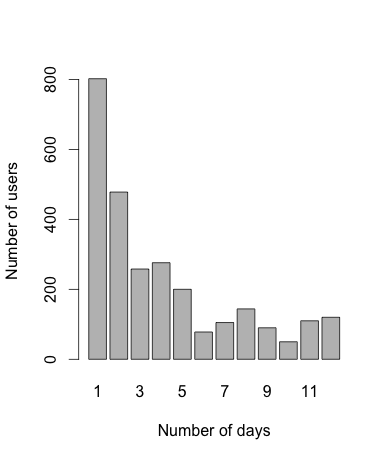
\includegraphics[width=\columnwidth]{imgs/Engagement2.png}
%  \end{center}
%\caption{Engagement - number of users/number of days}
%\label{img:Engagement-days}
%\end{figure}
%










\section{Conclusion}


\section{Future work}

\begin{itemize}
\item Setting up time/effort. 
\item Mix with contextual information. E.g. mobile phone data 
\item (we will find it out)
\end{itemize}



\bibliographystyle{plain}
\bibliography{references}
\end{document}
